\documentclass[a4paper]{article}
%\usepackage{graphicx}
\usepackage{amsmath}
\usepackage{svg}

\usepackage{geometry}
 \geometry{
 a4paper,
 total={150mm,257mm},
 top=20mm,
 }

\newcommand{\di}{i}

\begin{document}
\iffalse
Waveguide mit Gate in der Mitte?

NPN junction? 

Nächste Arbeitsschritte:
* Kurz LDOS untersuchen
* Integral für HB aufschreiben: NIntegrate? Überhaupt Intergrate?
* Integral für Hourglass setup aufschreiben, wie auswerten?
* Text in das LatexFile einfügen

Fragen, zur Vorbereitung:
* Was sind die Einheiten:
** Strom
** Leitfähigkeit
** Flux
** Potential

Jedes Kapitel: was willst du erzählen, was ist die Message? 

Wo siehst du Möglichkeiten, weiterzumachen?
\fi

\section{QPC}
\begin{figure}[h!]
\centering
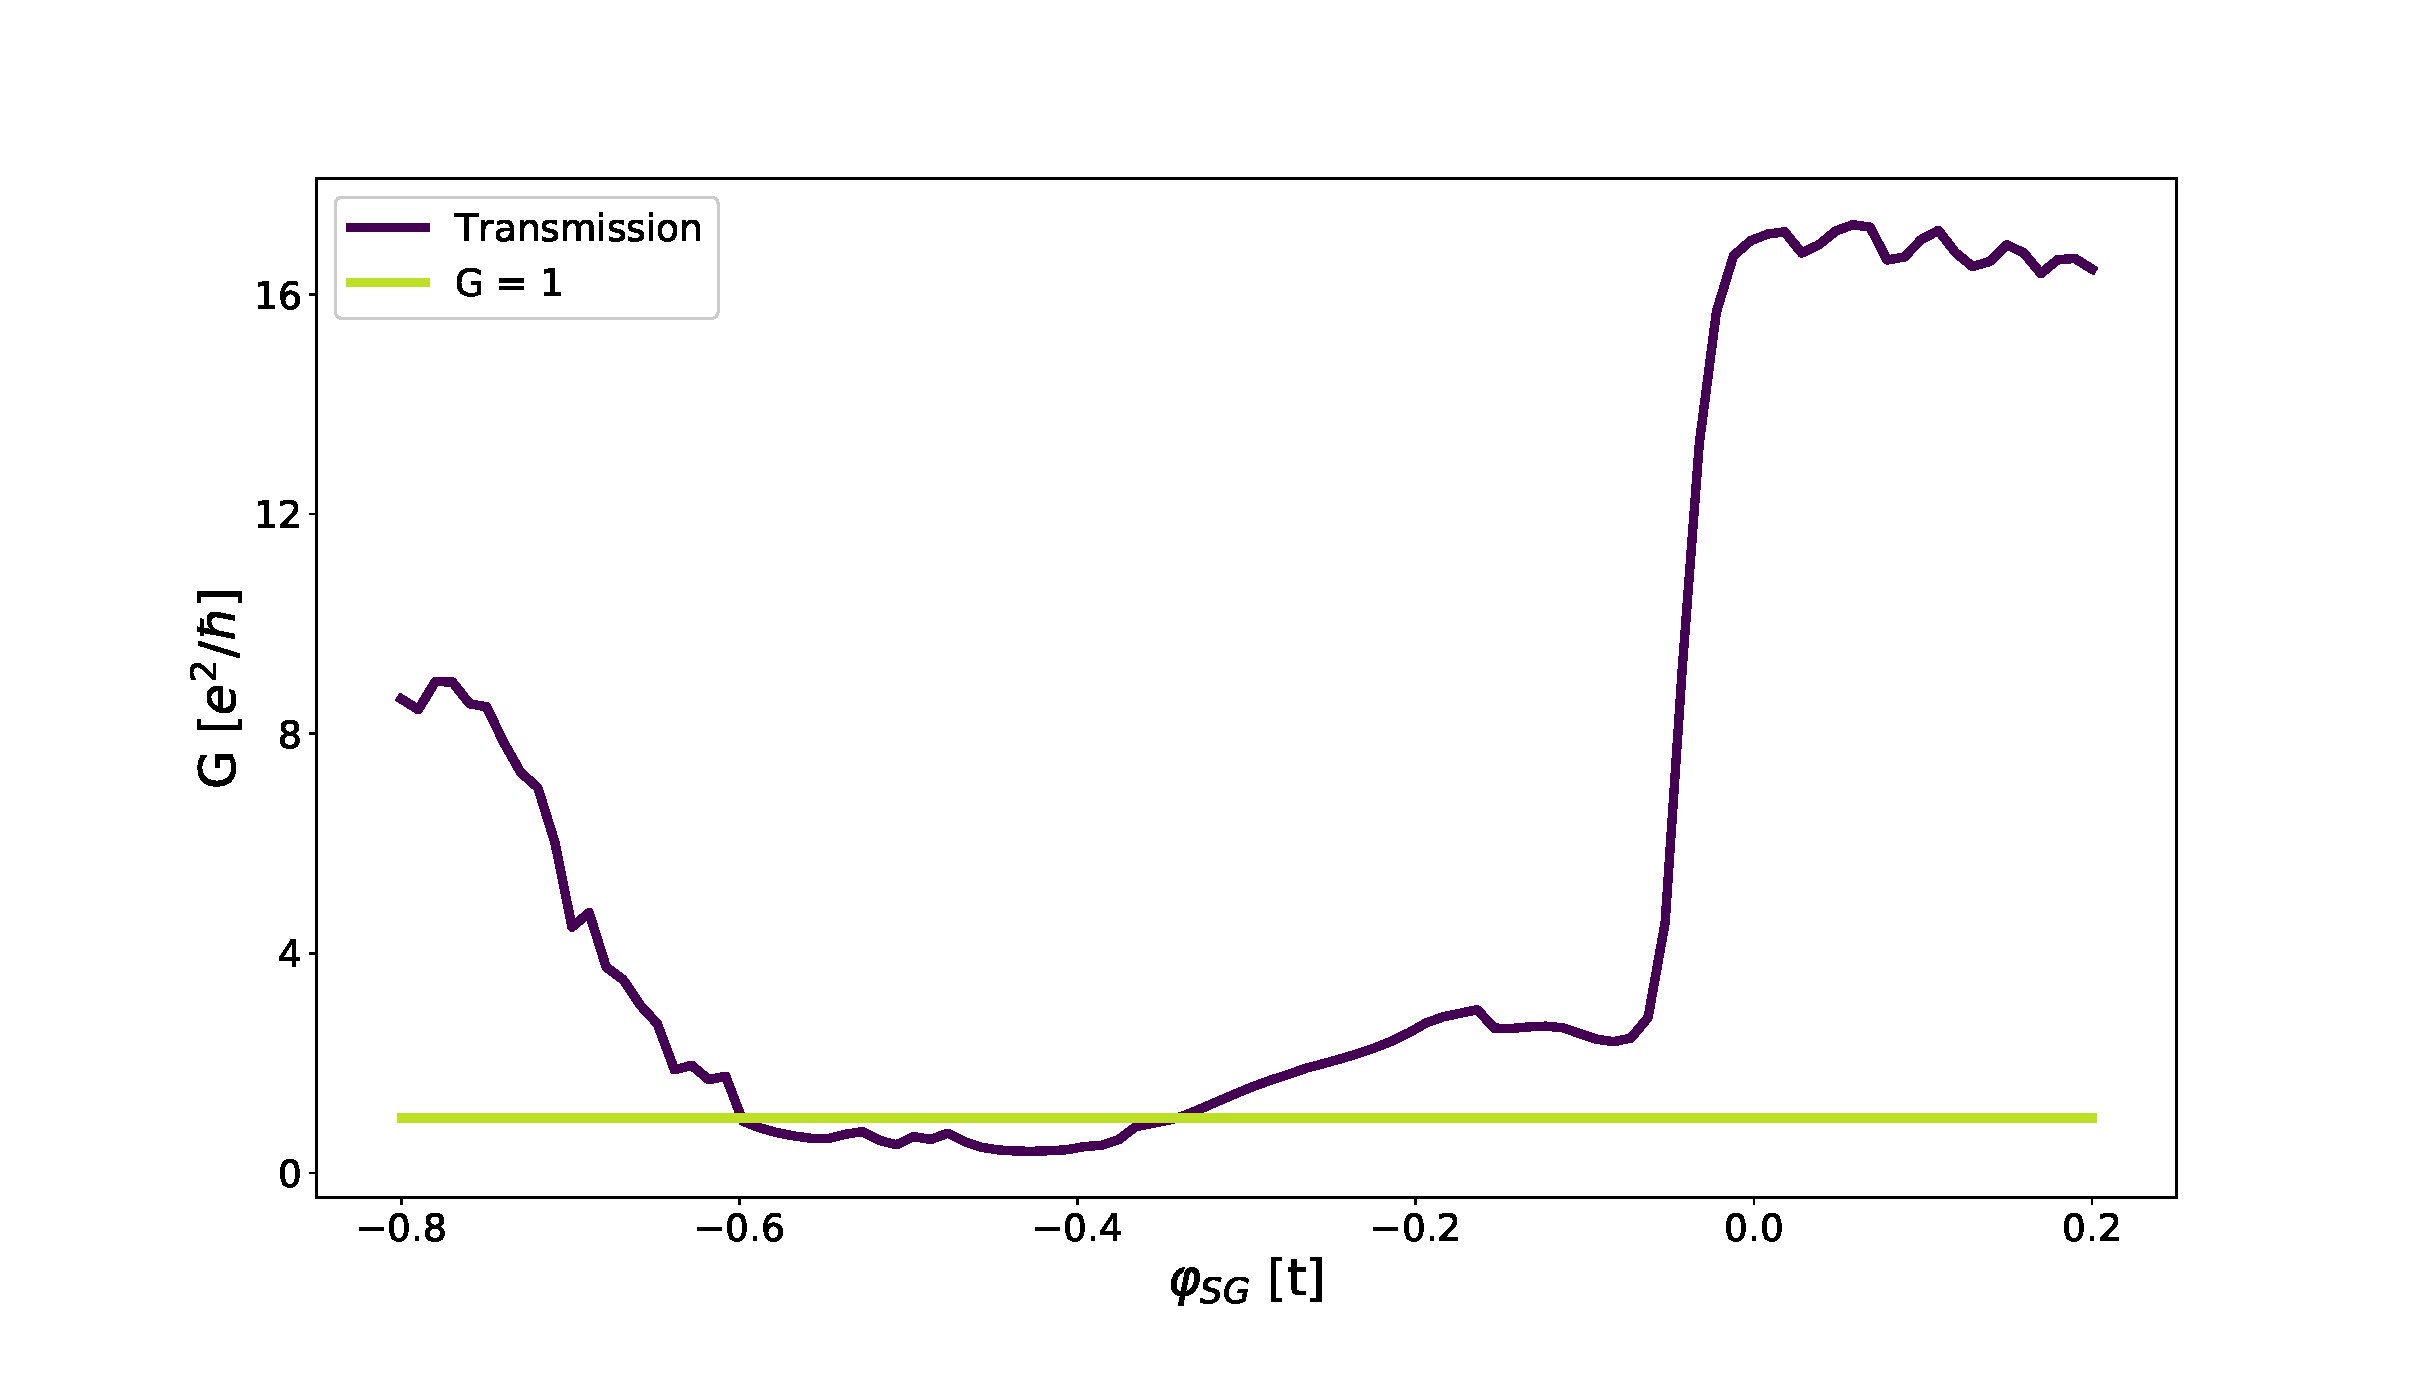
\includegraphics[width=0.8\textwidth]{qpc-conductance}
\caption{Conductance of QPC setup}
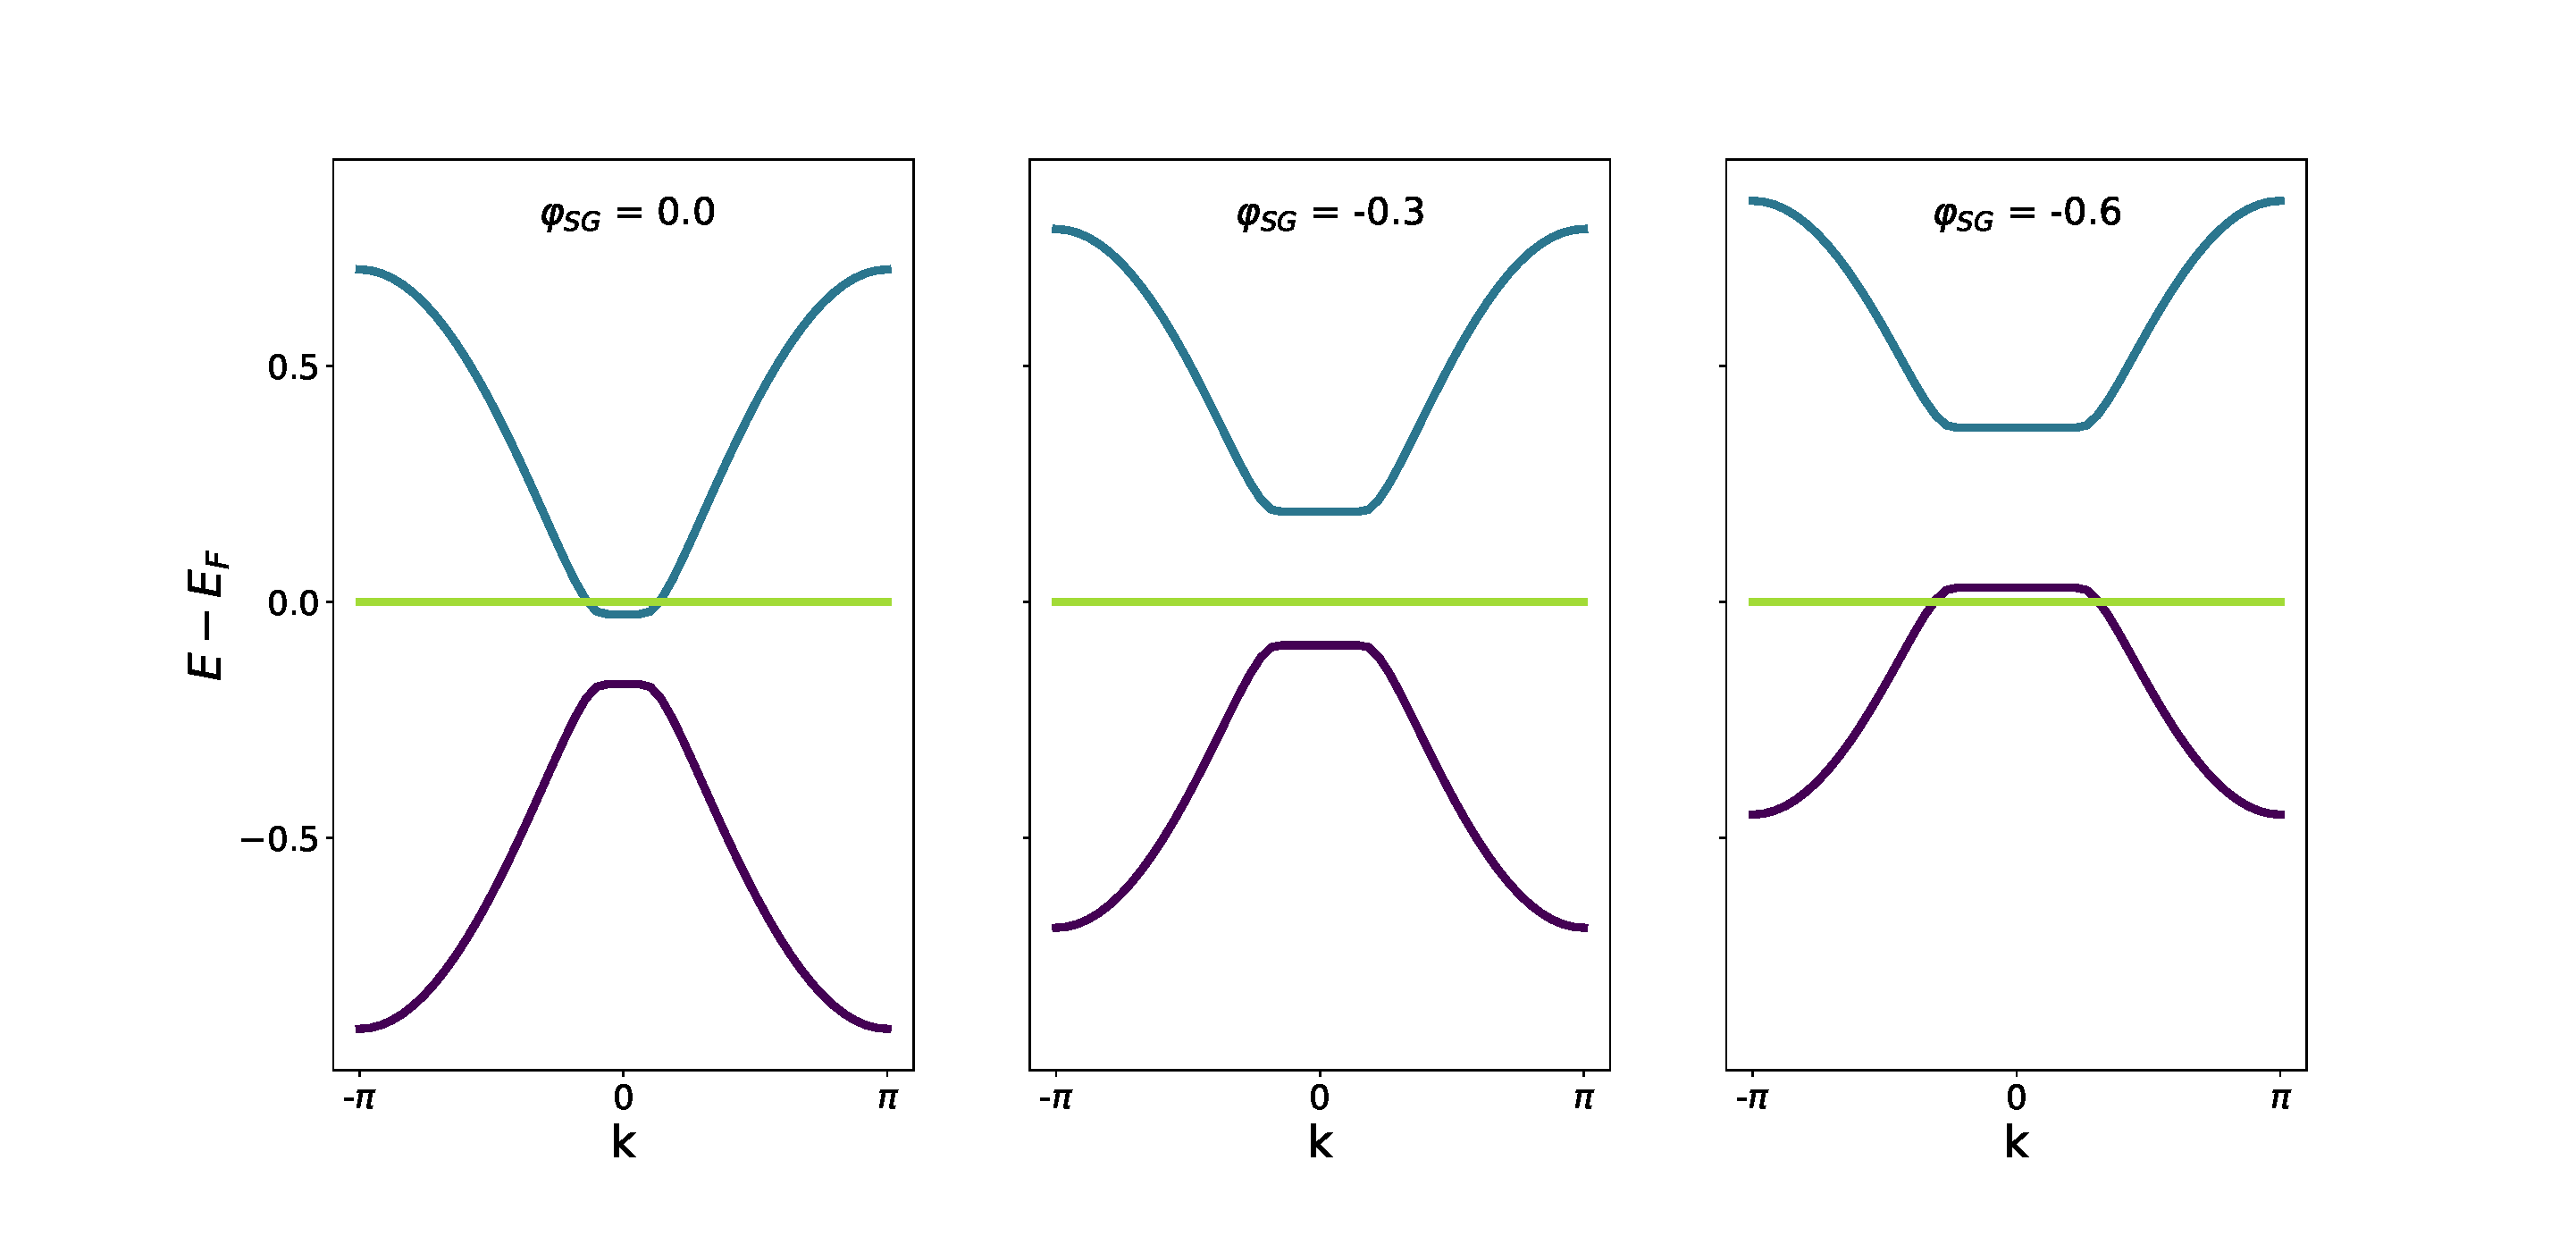
\includegraphics[width=0.8\textwidth]{bands-transition}
\caption{Bandstructure for different values of $\varphi_{SG}$ at constant $\varphi_{BG}$. Yellowish line marks $E_F - E = 0$}
\end{figure}
\begin{figure}
\centering
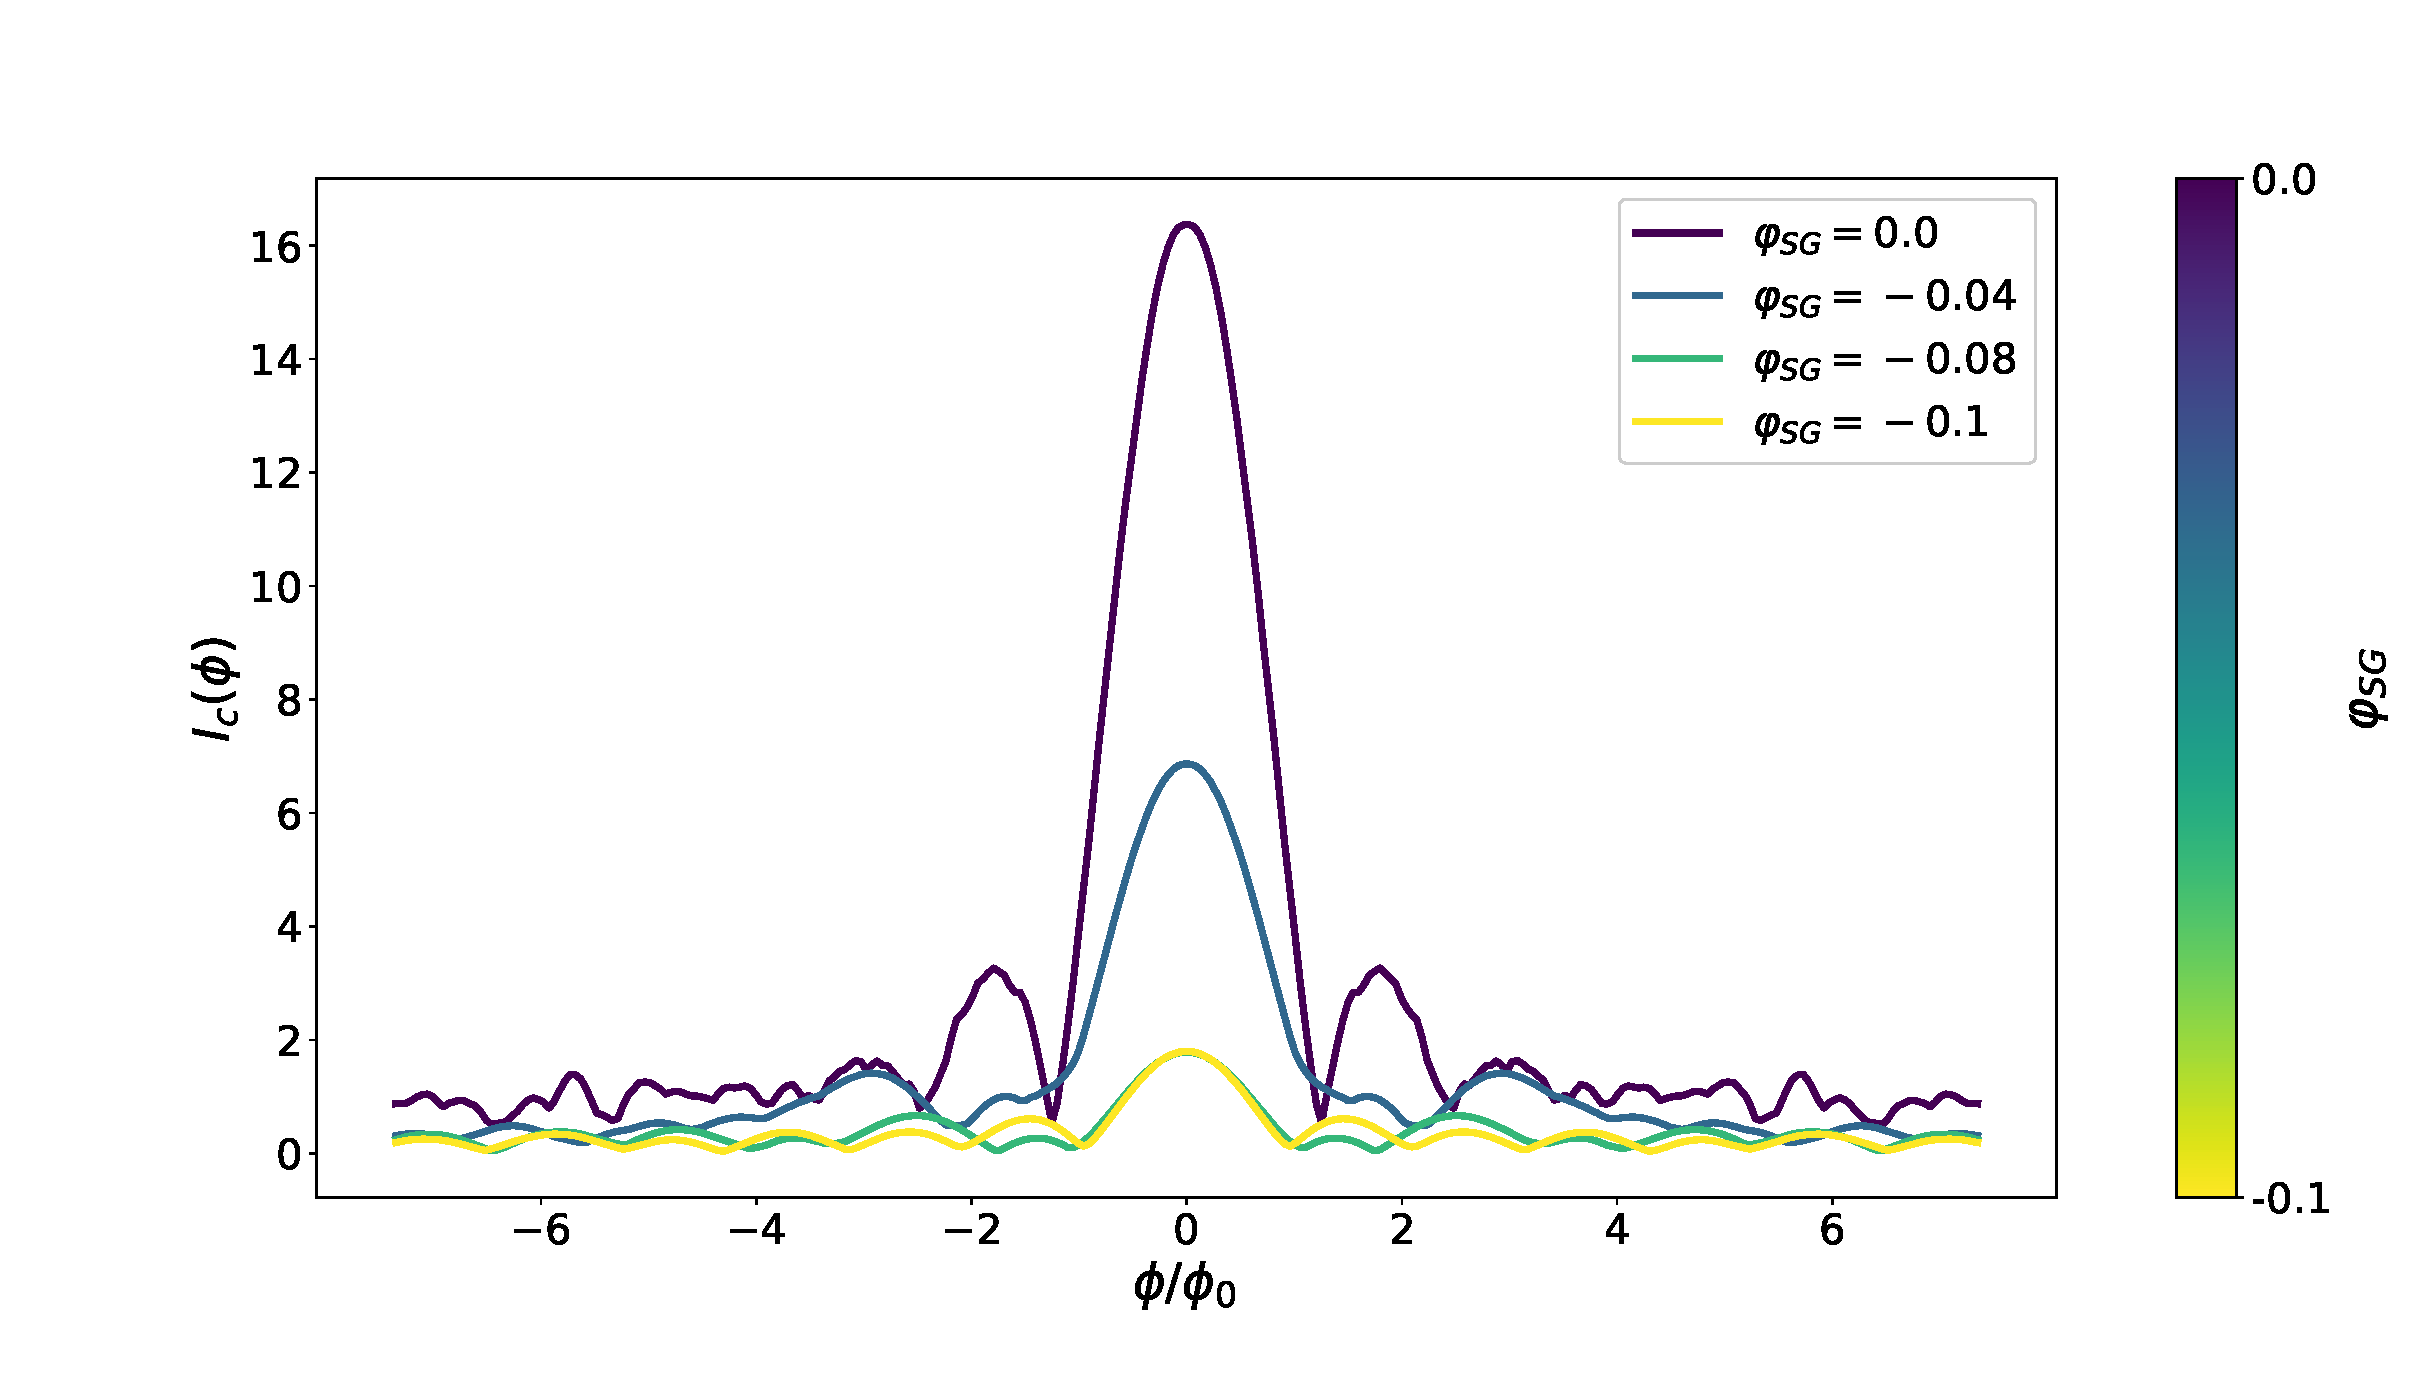
\includegraphics[width=0.8\textwidth]{qpc-0-01}
\caption{Supercurrent with increasing splitgate: $\varphi_{SG} \in [0.0, -0.1]$: transition from beating pattern to pattern for confined regime.}
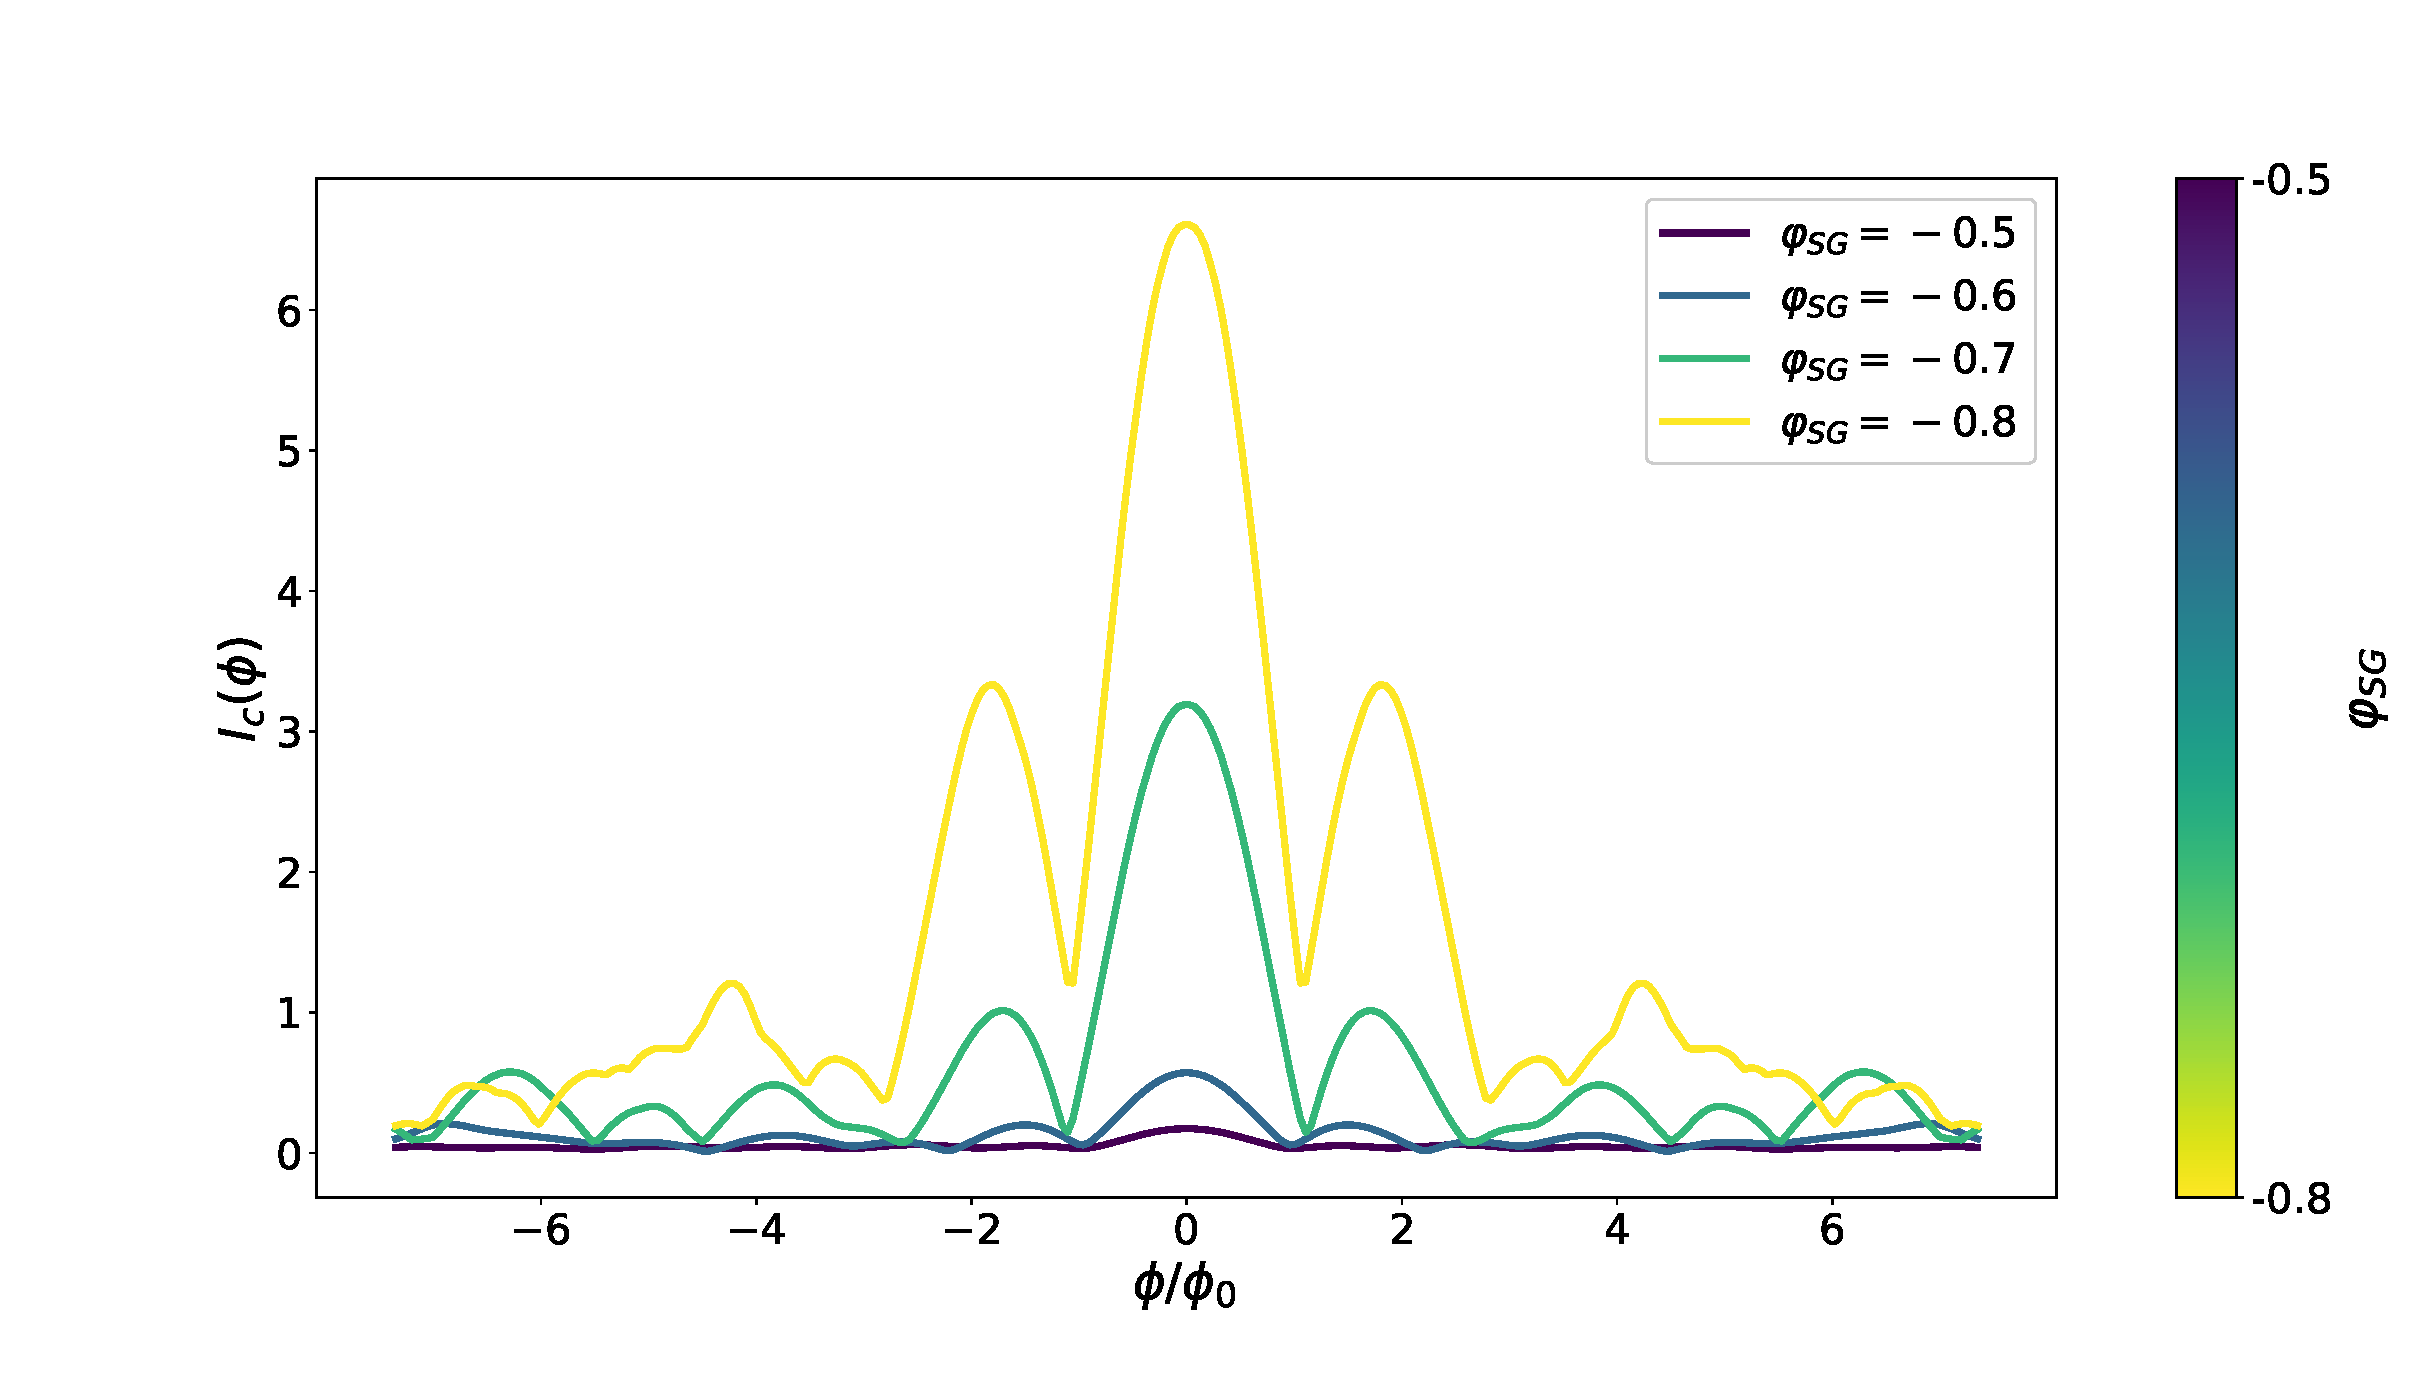
\includegraphics[width=0.8\textwidth]{qpc-05-08}
\caption{Supercurrent with increasing splitgate: $\varphi_{SG} \in [-0.5, -0.8]$: beating pattern recovers for increasing splitgate.}
\end{figure}

\newpage

\section{QPC with edge channels}

\begin{figure}[h!]
\centering
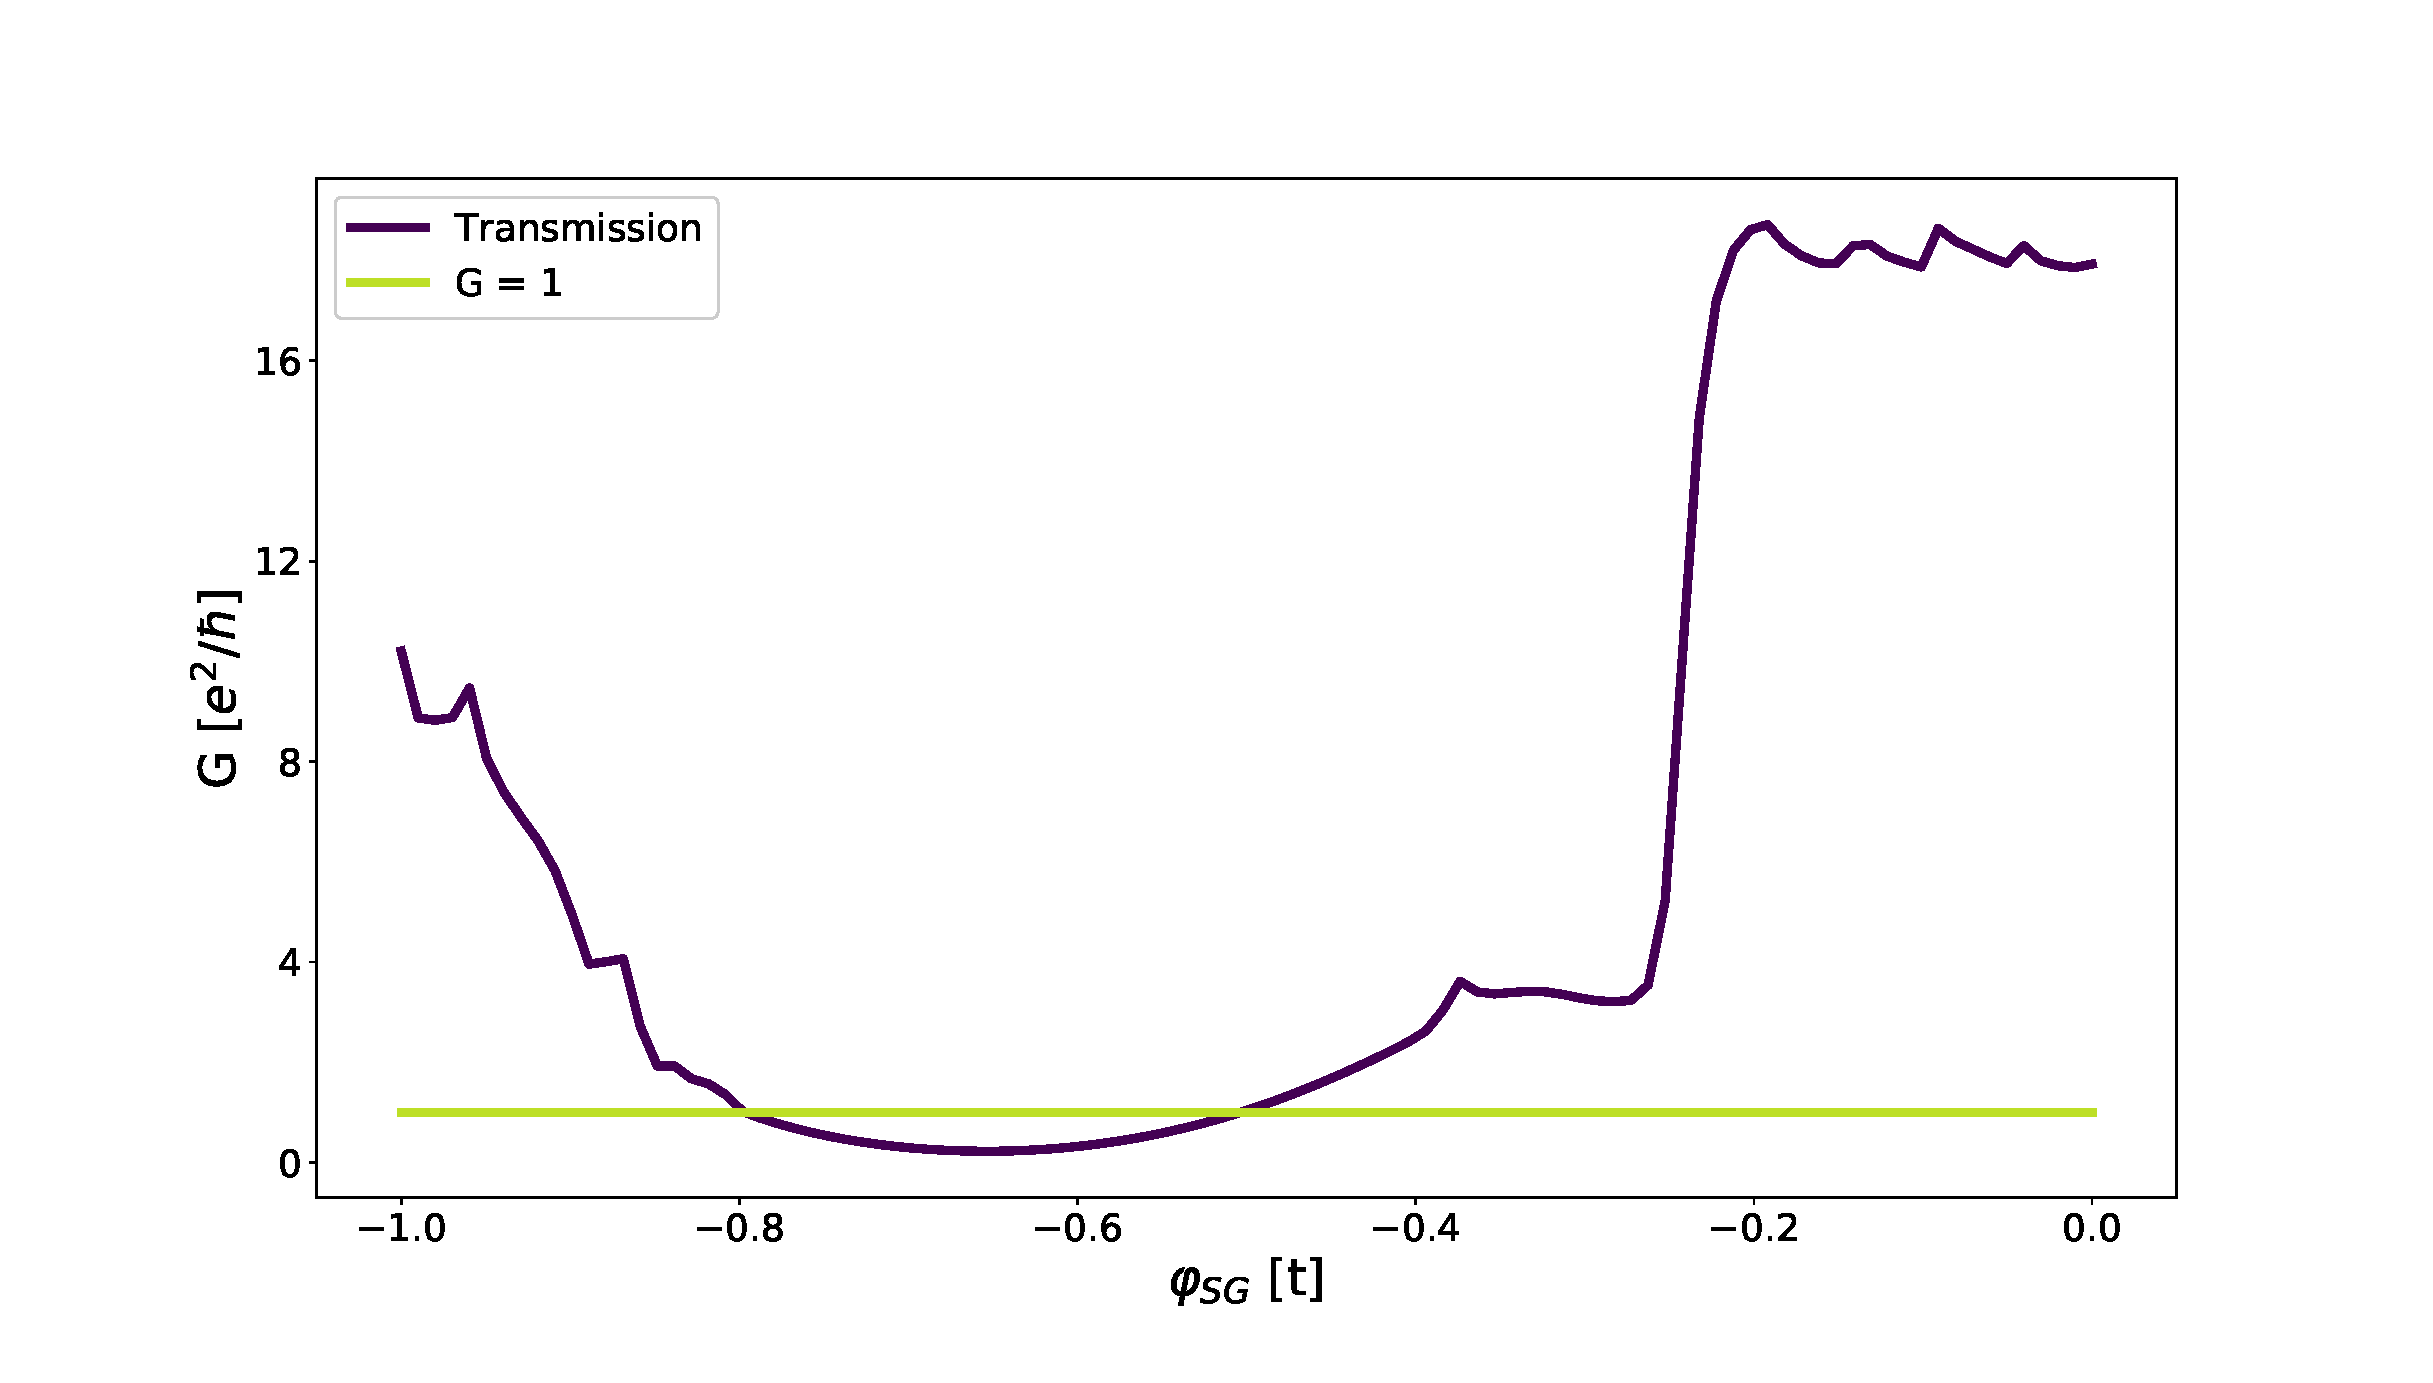
\includegraphics[width=0.8\textwidth]{qpc-edges-conductance}
\caption{Conductance of QPC-like setup with edge channels}
\end{figure}

\begin{figure}[h!]
\centering
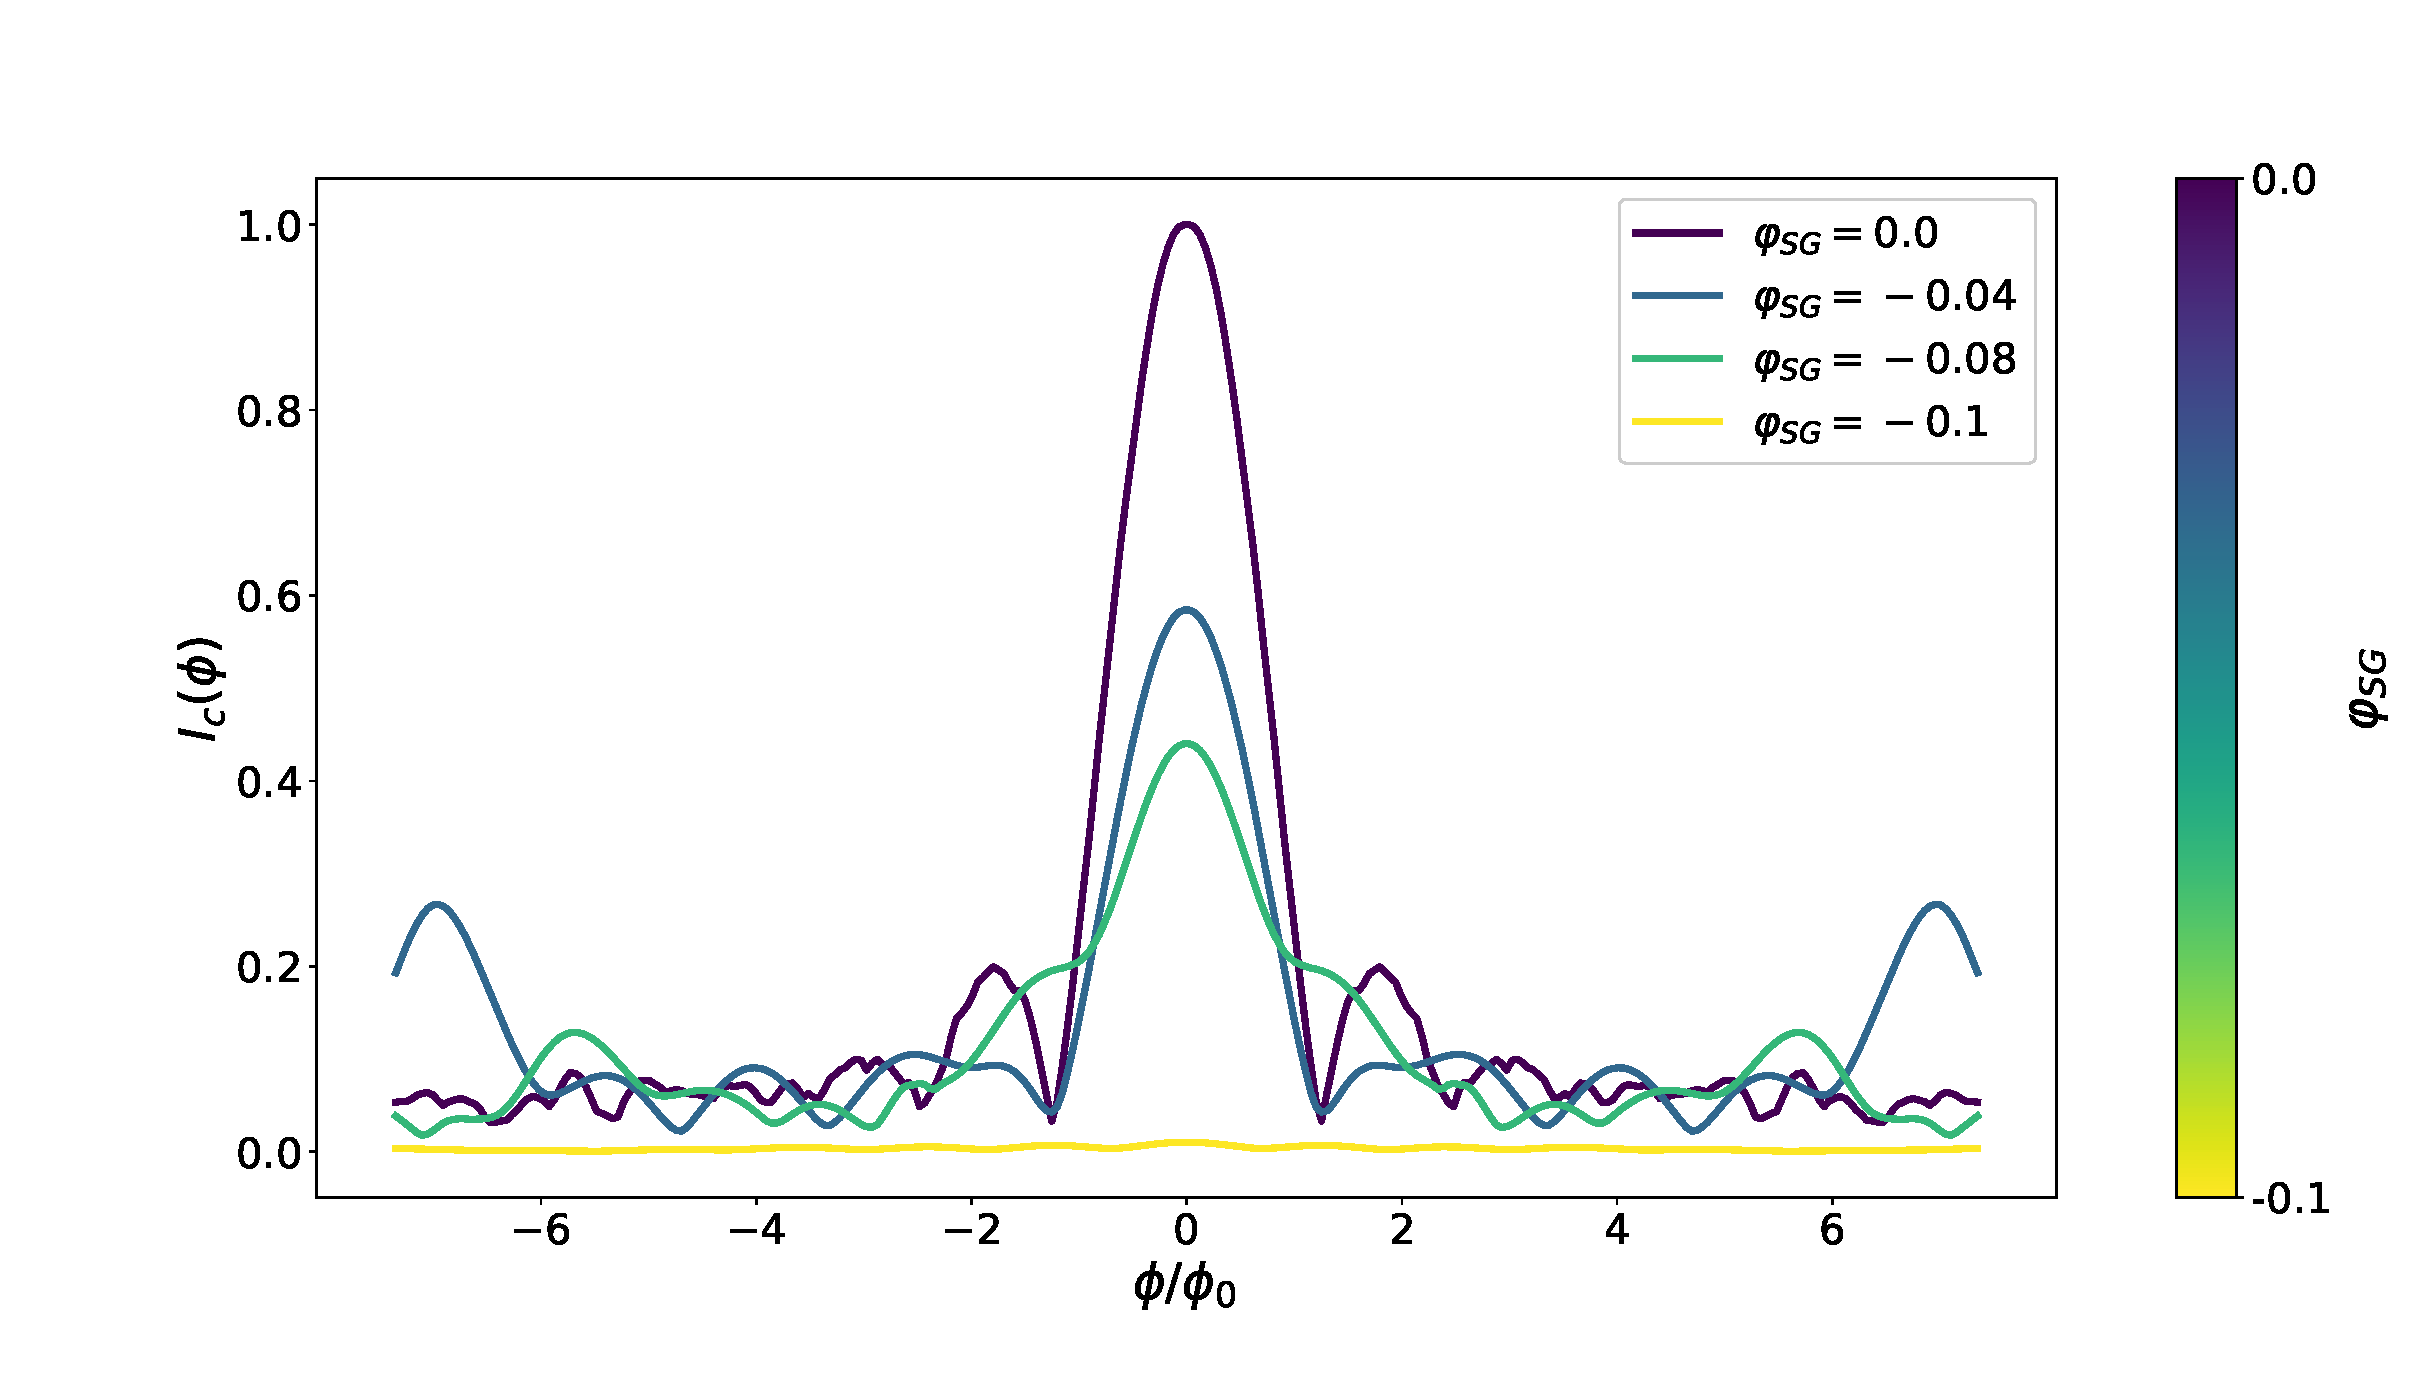
\includegraphics[width=0.8\textwidth]{qpc-edges-0-01}
\caption{Supercurrent with increasing splitgate: $\varphi_{SG} \in [0.0, -0.1]$}
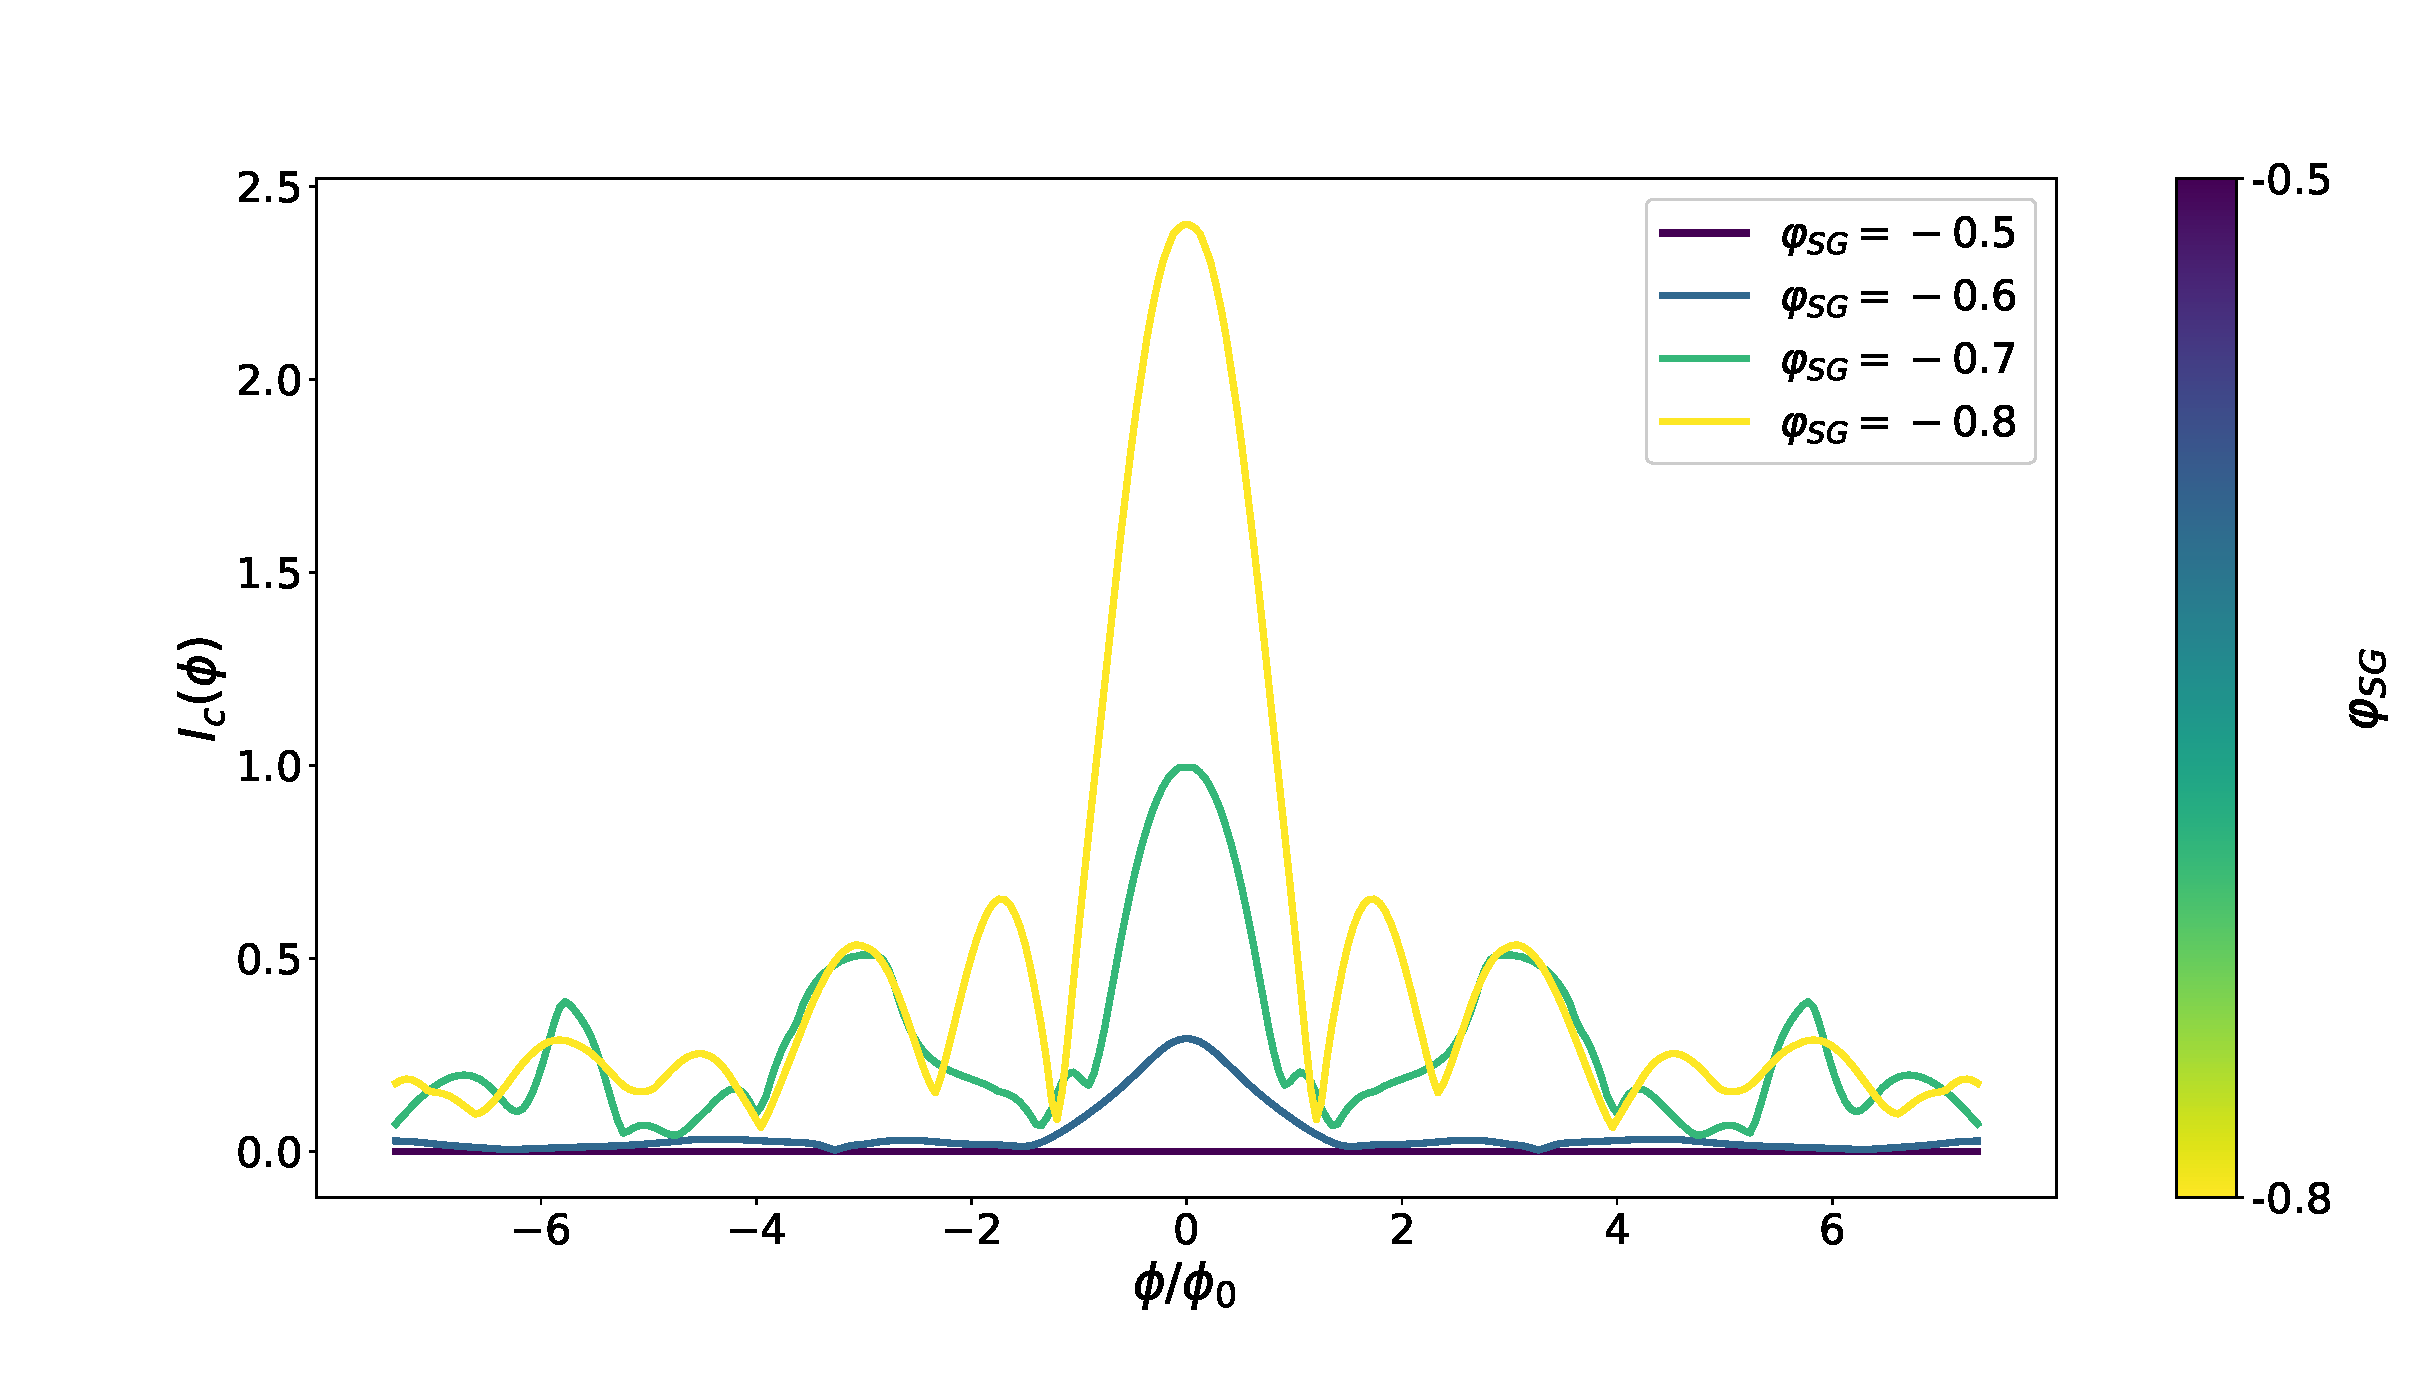
\includegraphics[width=0.8\textwidth]{qpc-edges-05-08}
\caption{Supercurrent with increasing splitgate: $\varphi_{SG} \in [-0.5, -0.8]$}
\end{figure}

\newpage
\section{Half barrier setup}
\begin{figure}[h!]
\centering
\begin{minipage}{0.3\textwidth}
\centering
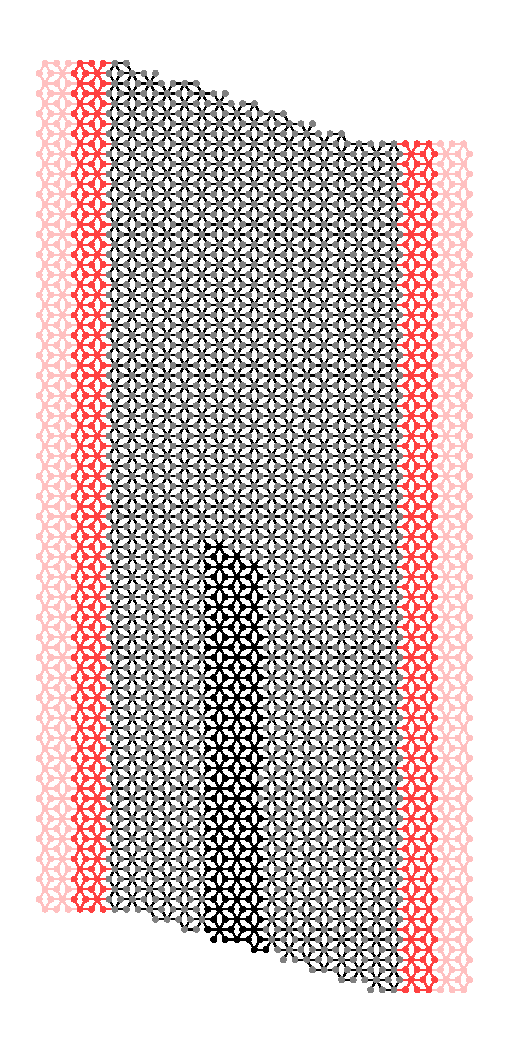
\includegraphics[width=0.6\textwidth]{hb_lower}
\caption{Lower finger}
\end{minipage}%
\begin{minipage}{0.7\textwidth}
\centering
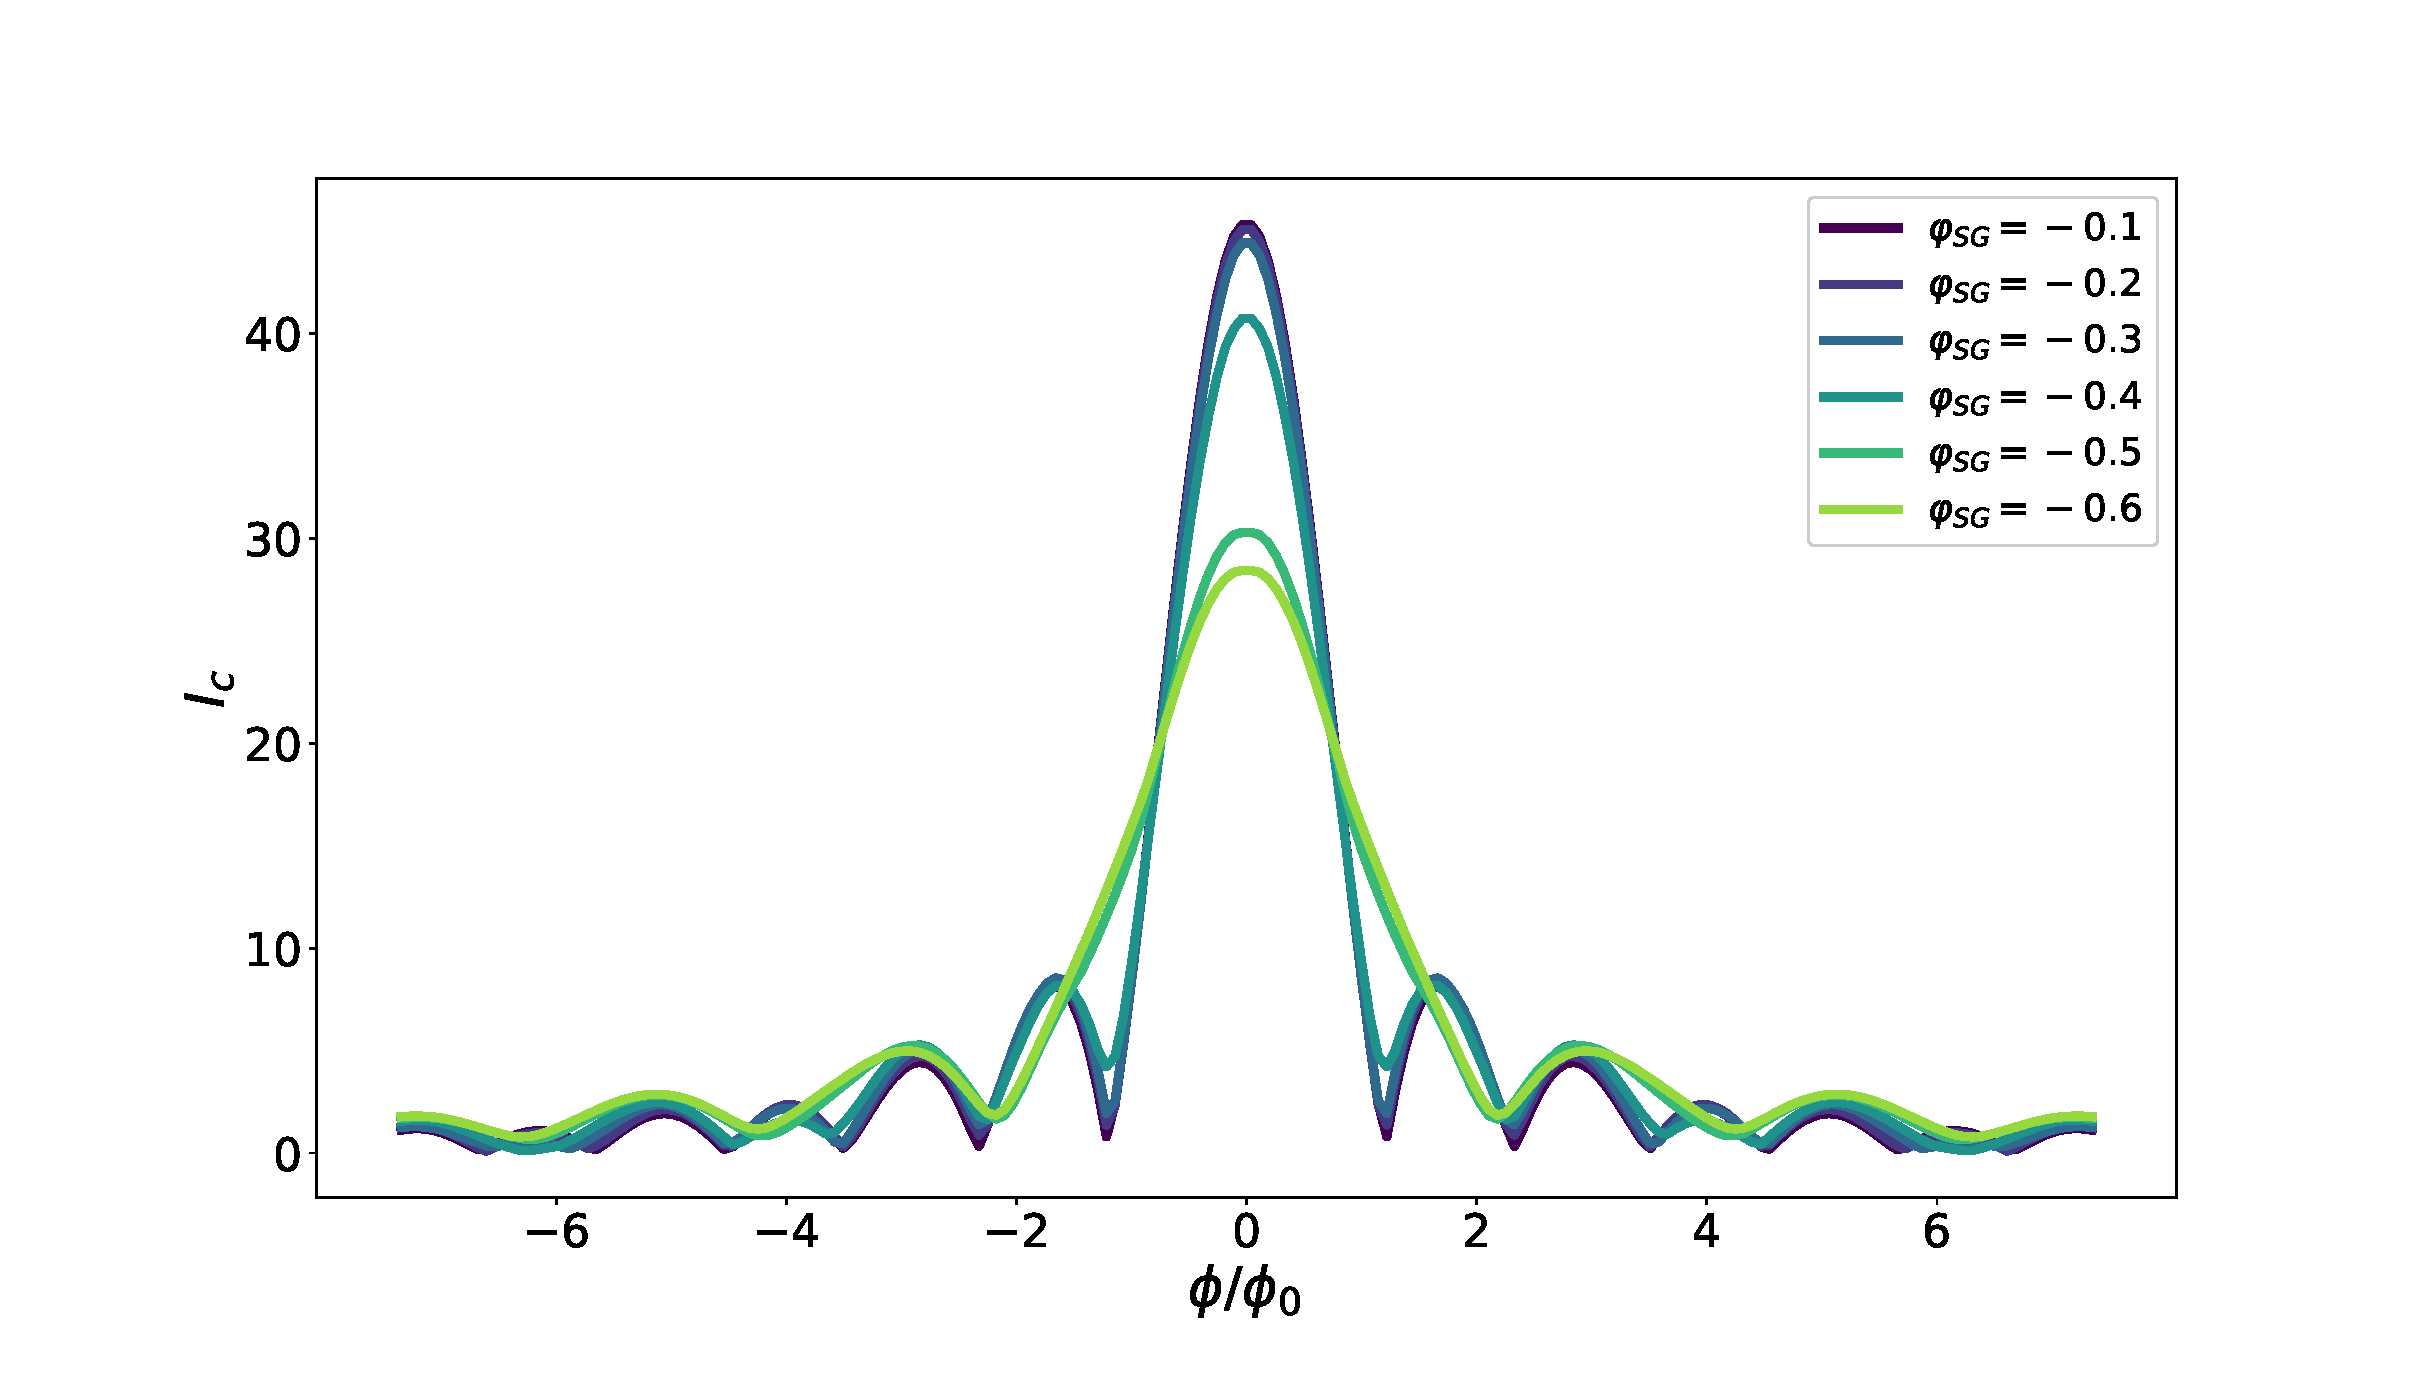
\includegraphics[width=\textwidth]{hb_lower_plot}
\caption{Critical current of lower finger}
\end{minipage}
\end{figure}
\begin{figure}[h!]
\centering
\begin{minipage}{0.3\textwidth}
\centering
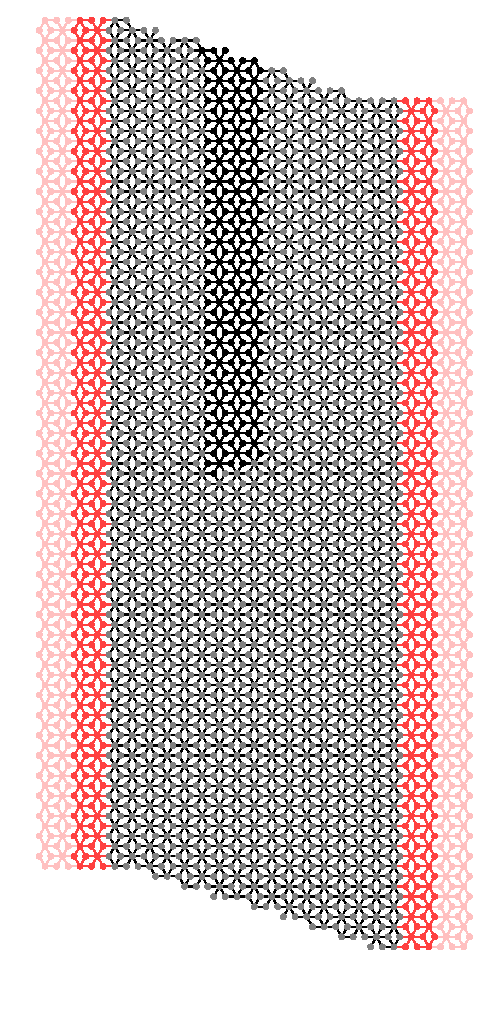
\includegraphics[width=0.6\textwidth]{hb_upper}
\caption{Upper finger}
\end{minipage}%
\begin{minipage}{0.7\textwidth}
\centering
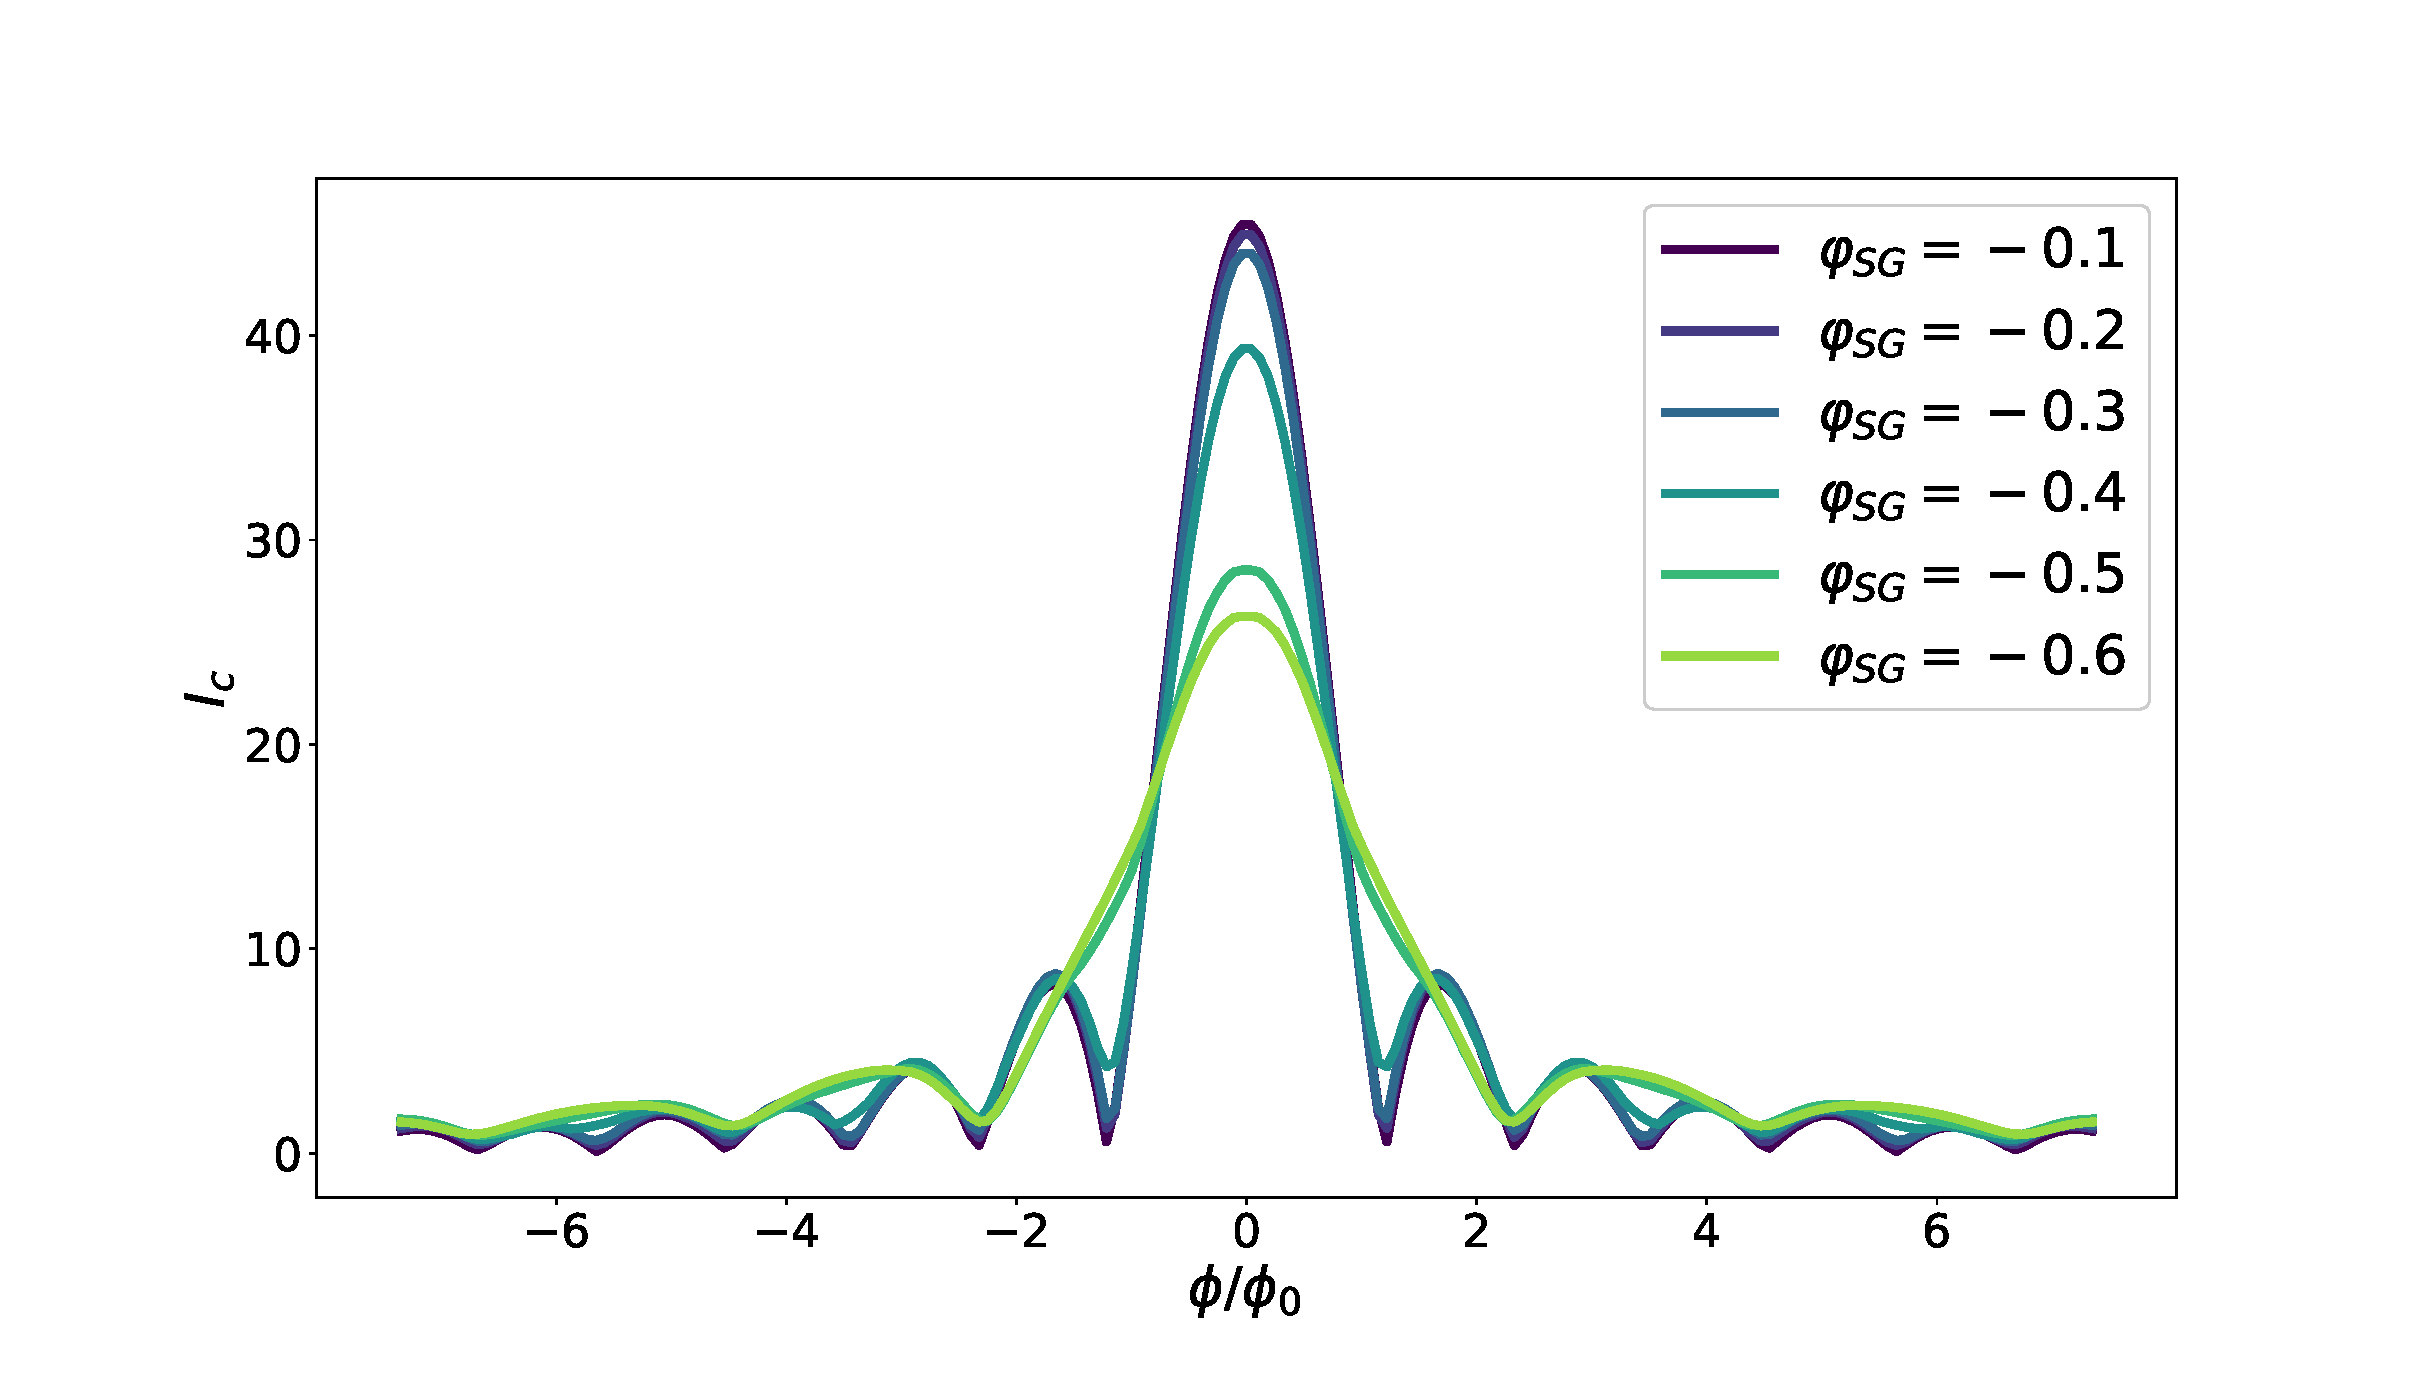
\includegraphics[width=\textwidth]{hb_upper_plot}
\caption{Critical current of upper finger}
\end{minipage}
\end{figure}
\begin{figure}[h!]
\centering
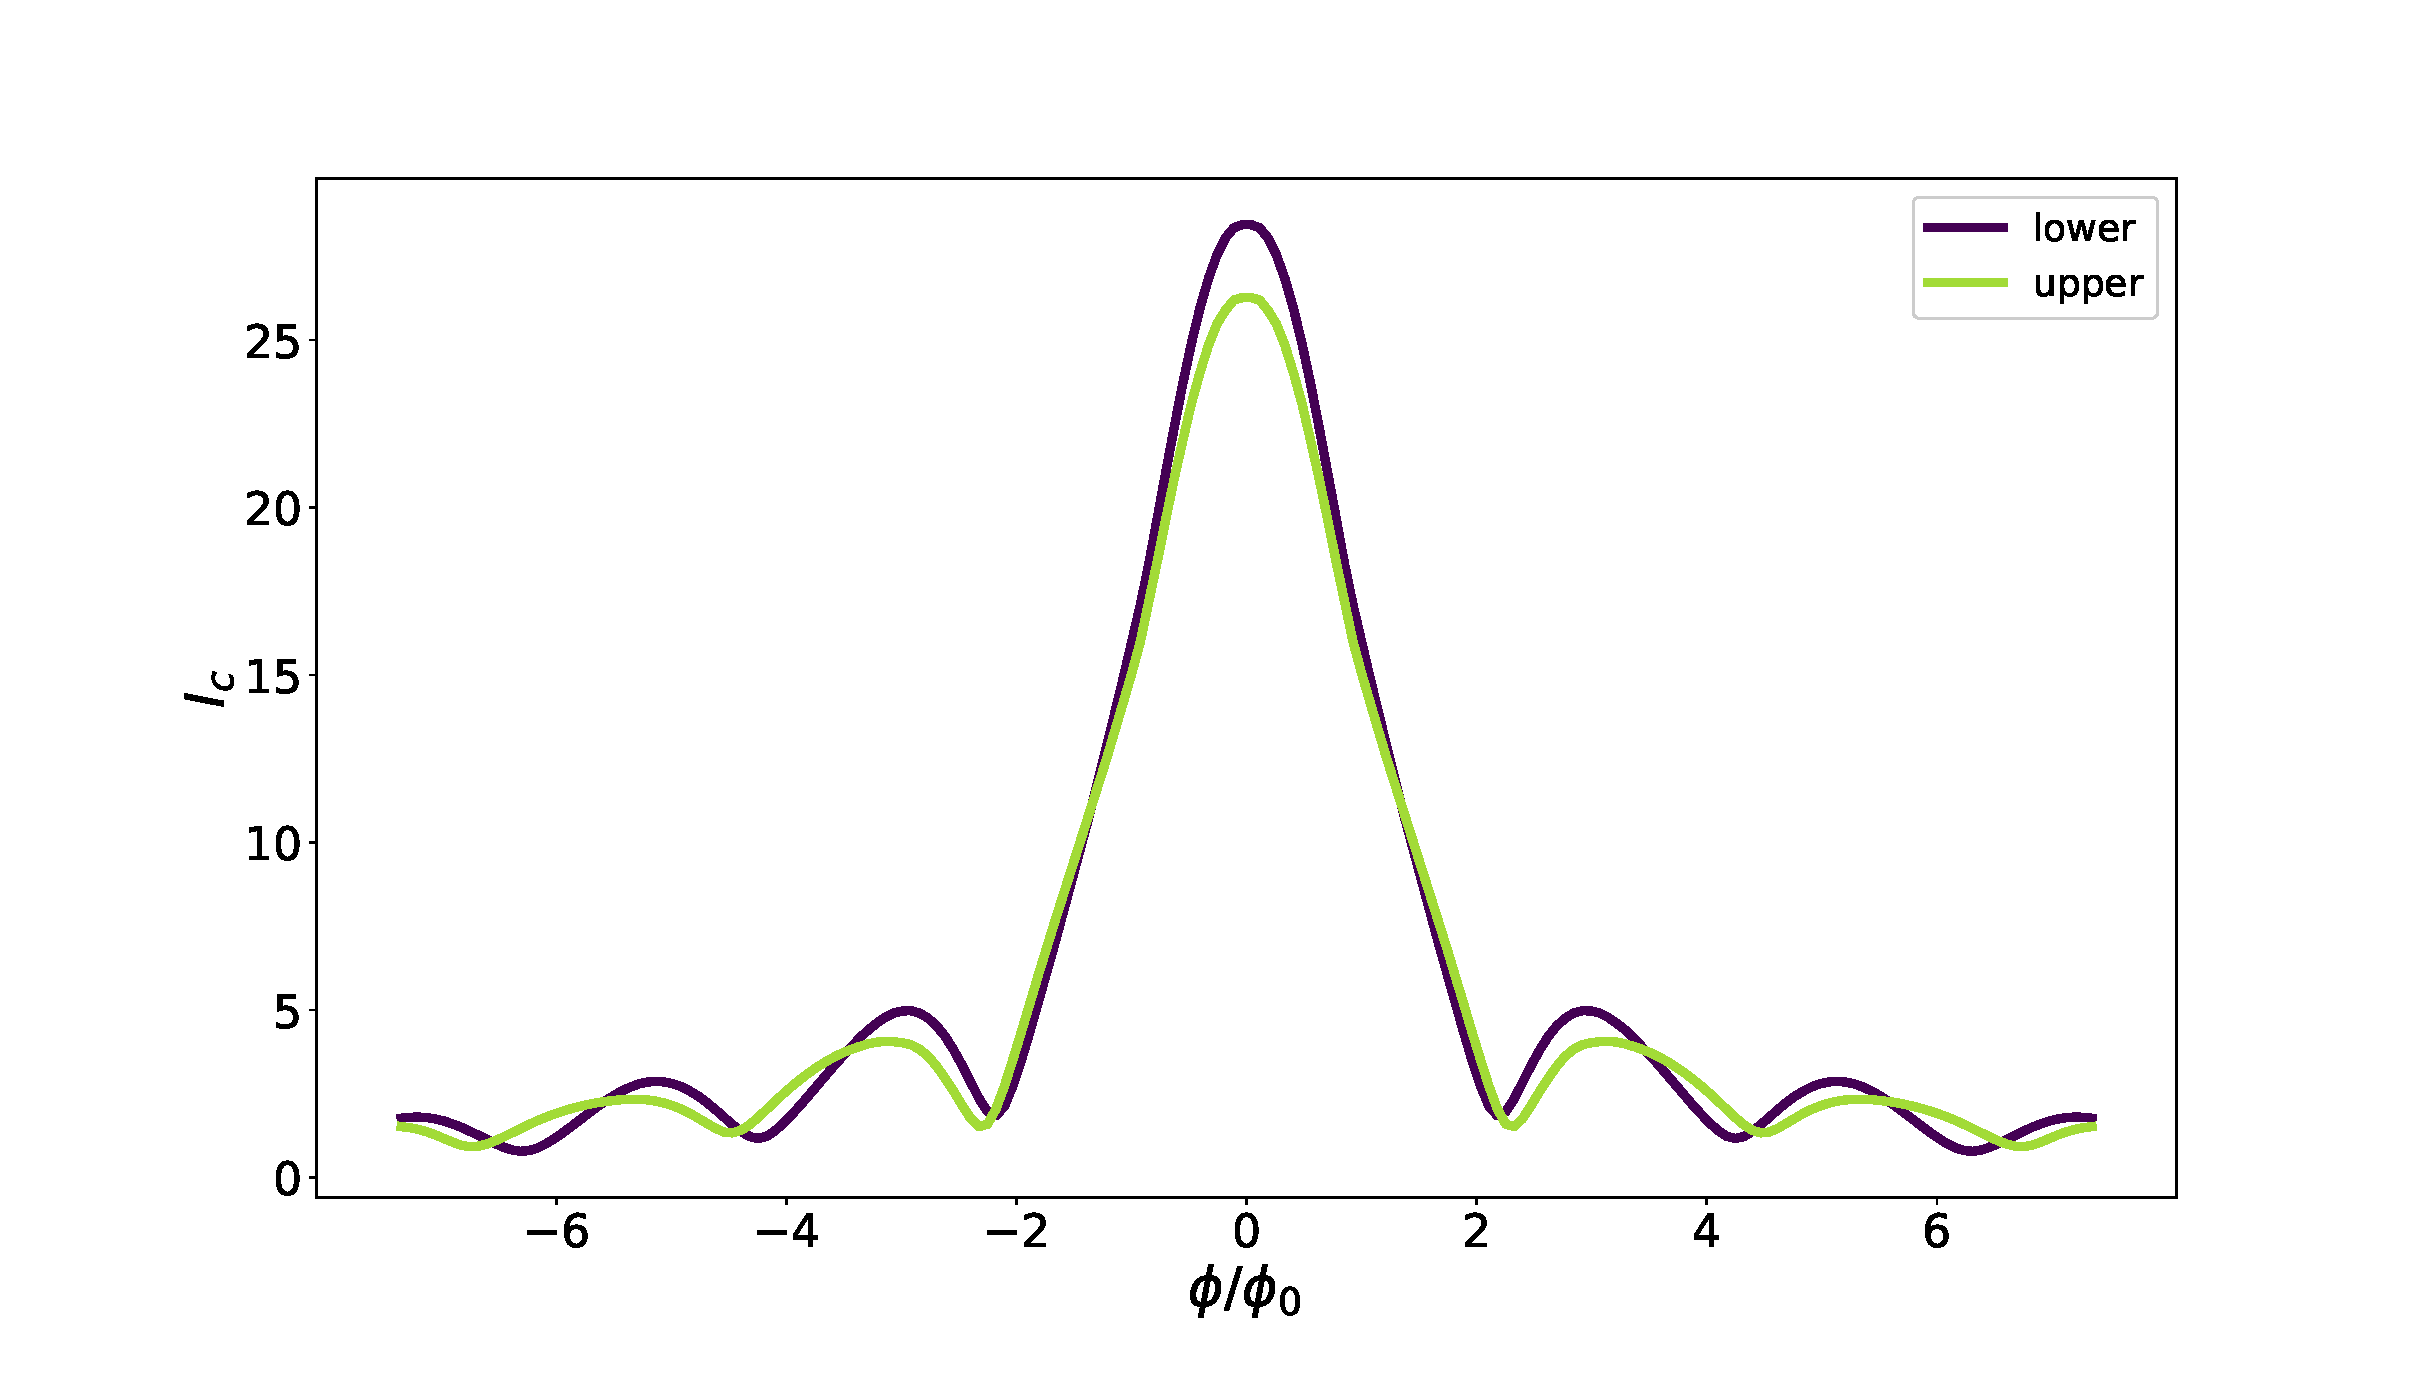
\includegraphics[width=0.8\textwidth]{hb_comparison}
\caption{Comparing critical current curves for upper and lower finger of constriction at the same topgate voltage}
\end{figure}
\newpage

\section{Waveguide}
\iffalse
Less impact of stray fields

What could be done and has not been evaluated so far:
* impact of disorder in the sample or in the leads
* finite doping in the leads
\fi

\begin{figure}[h!]
\centering
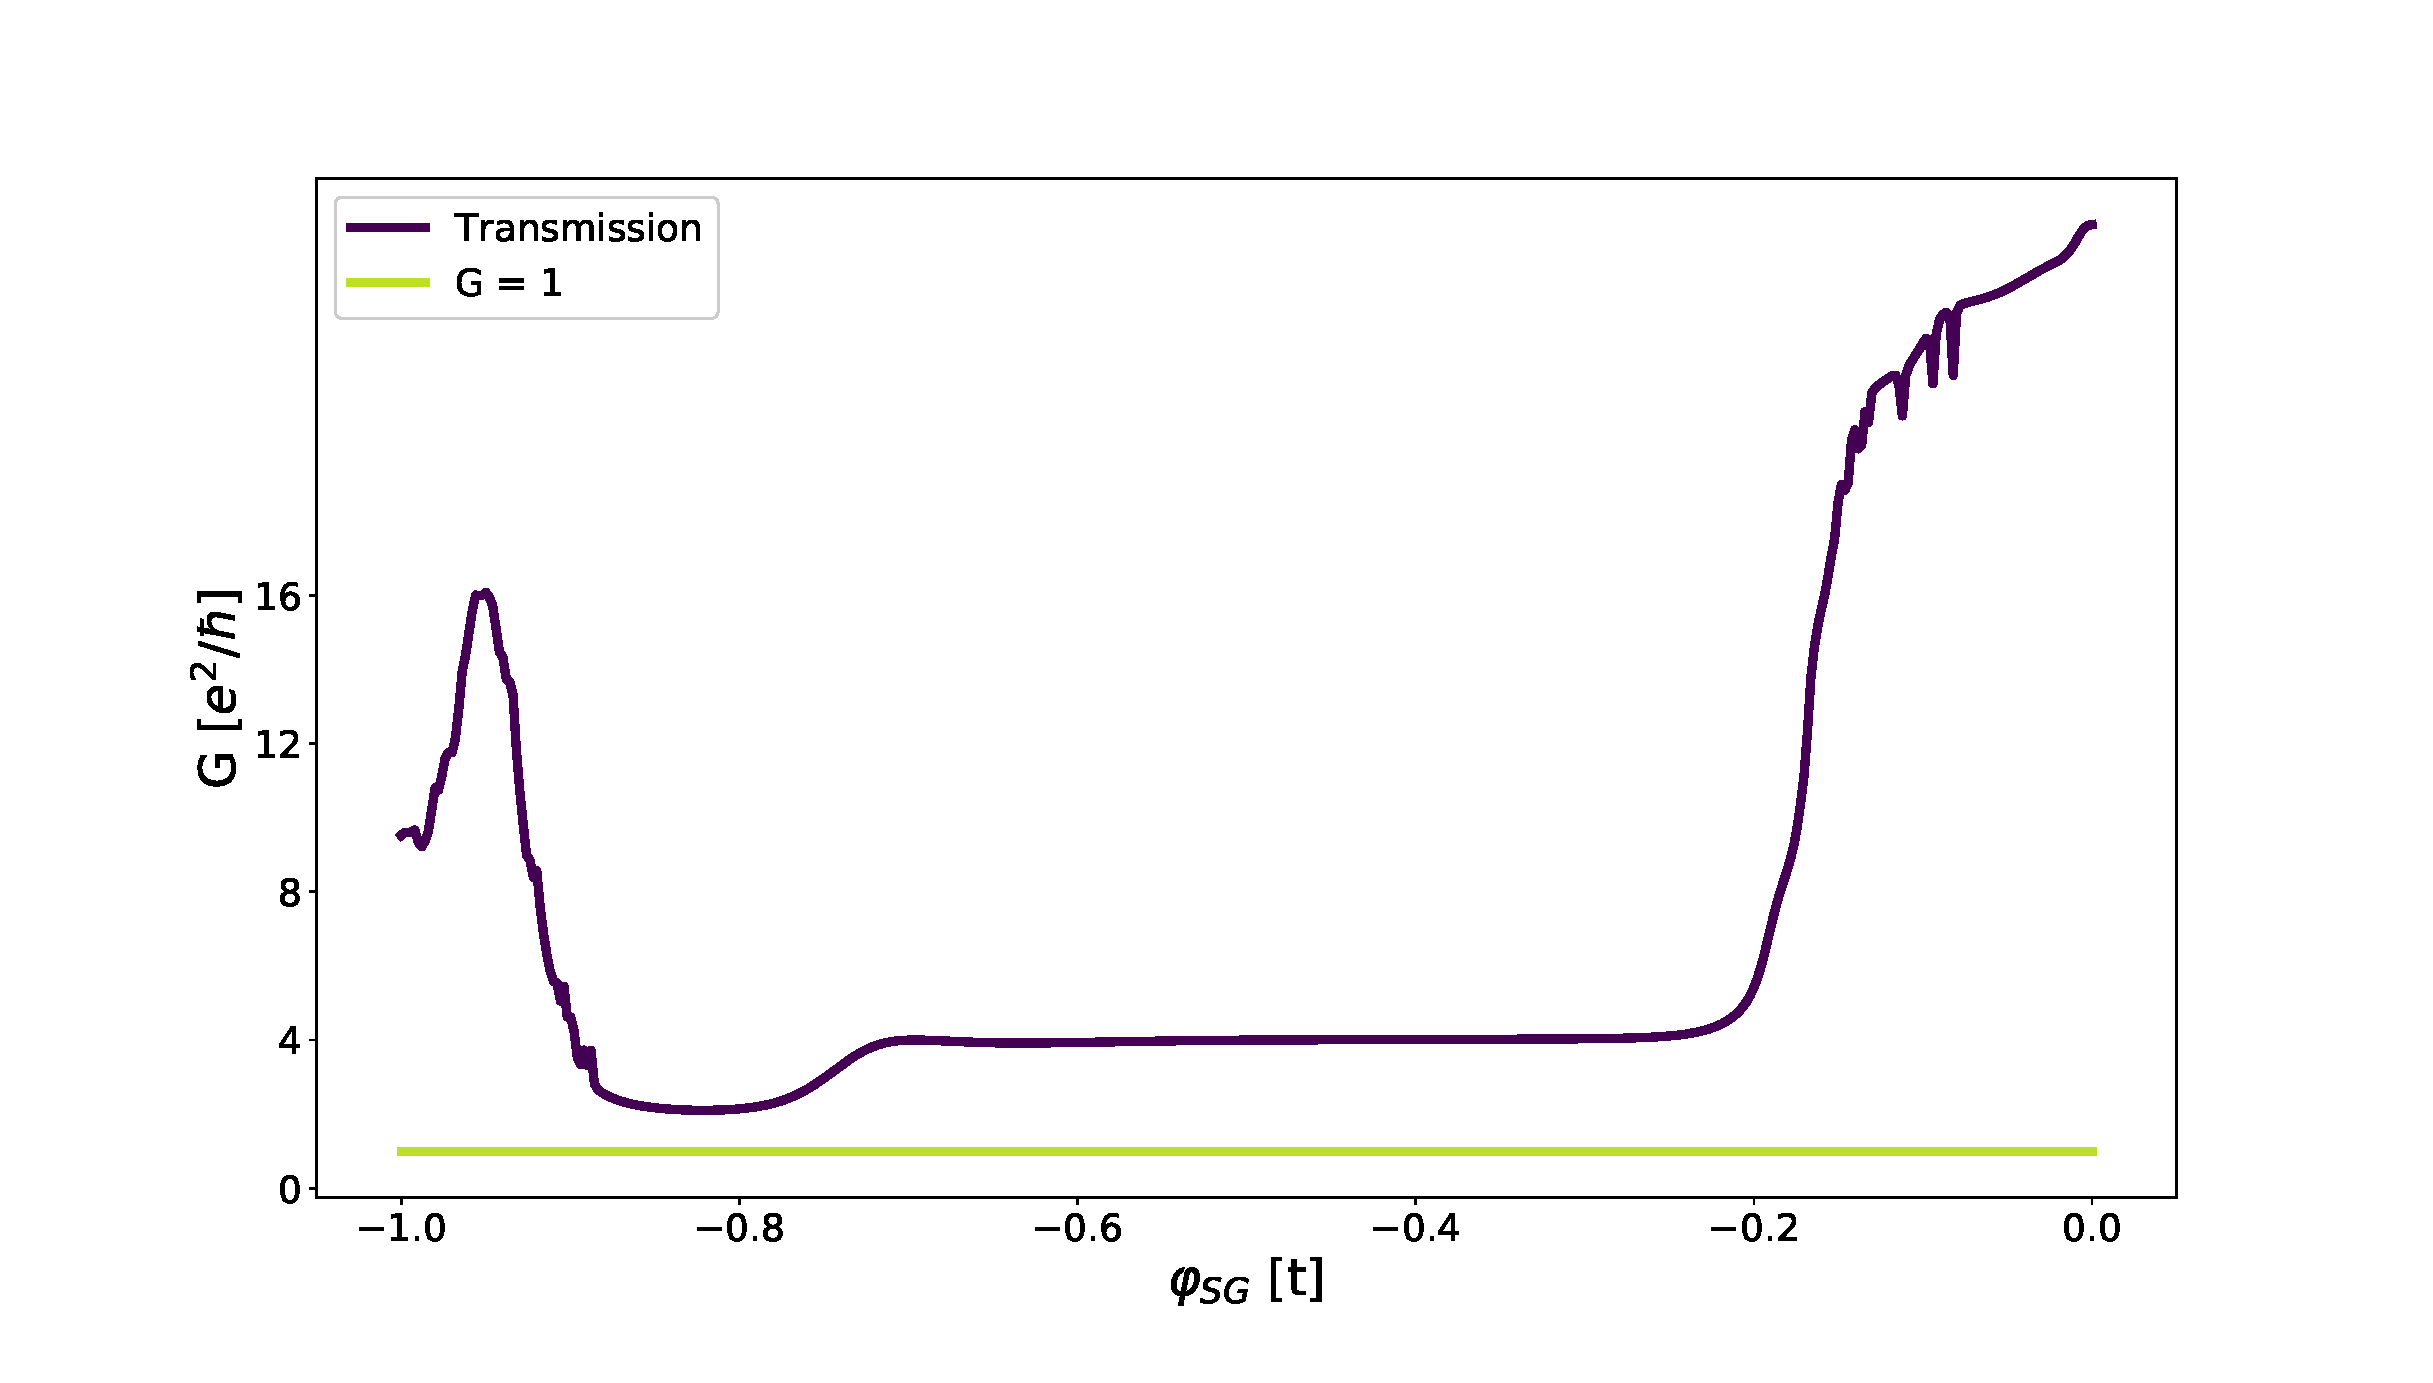
\includegraphics[width=0.8\textwidth]{wg-conductance}
\caption{Conductance of waveguide set-up}
\end{figure}

\begin{figure}[h!]
\centering
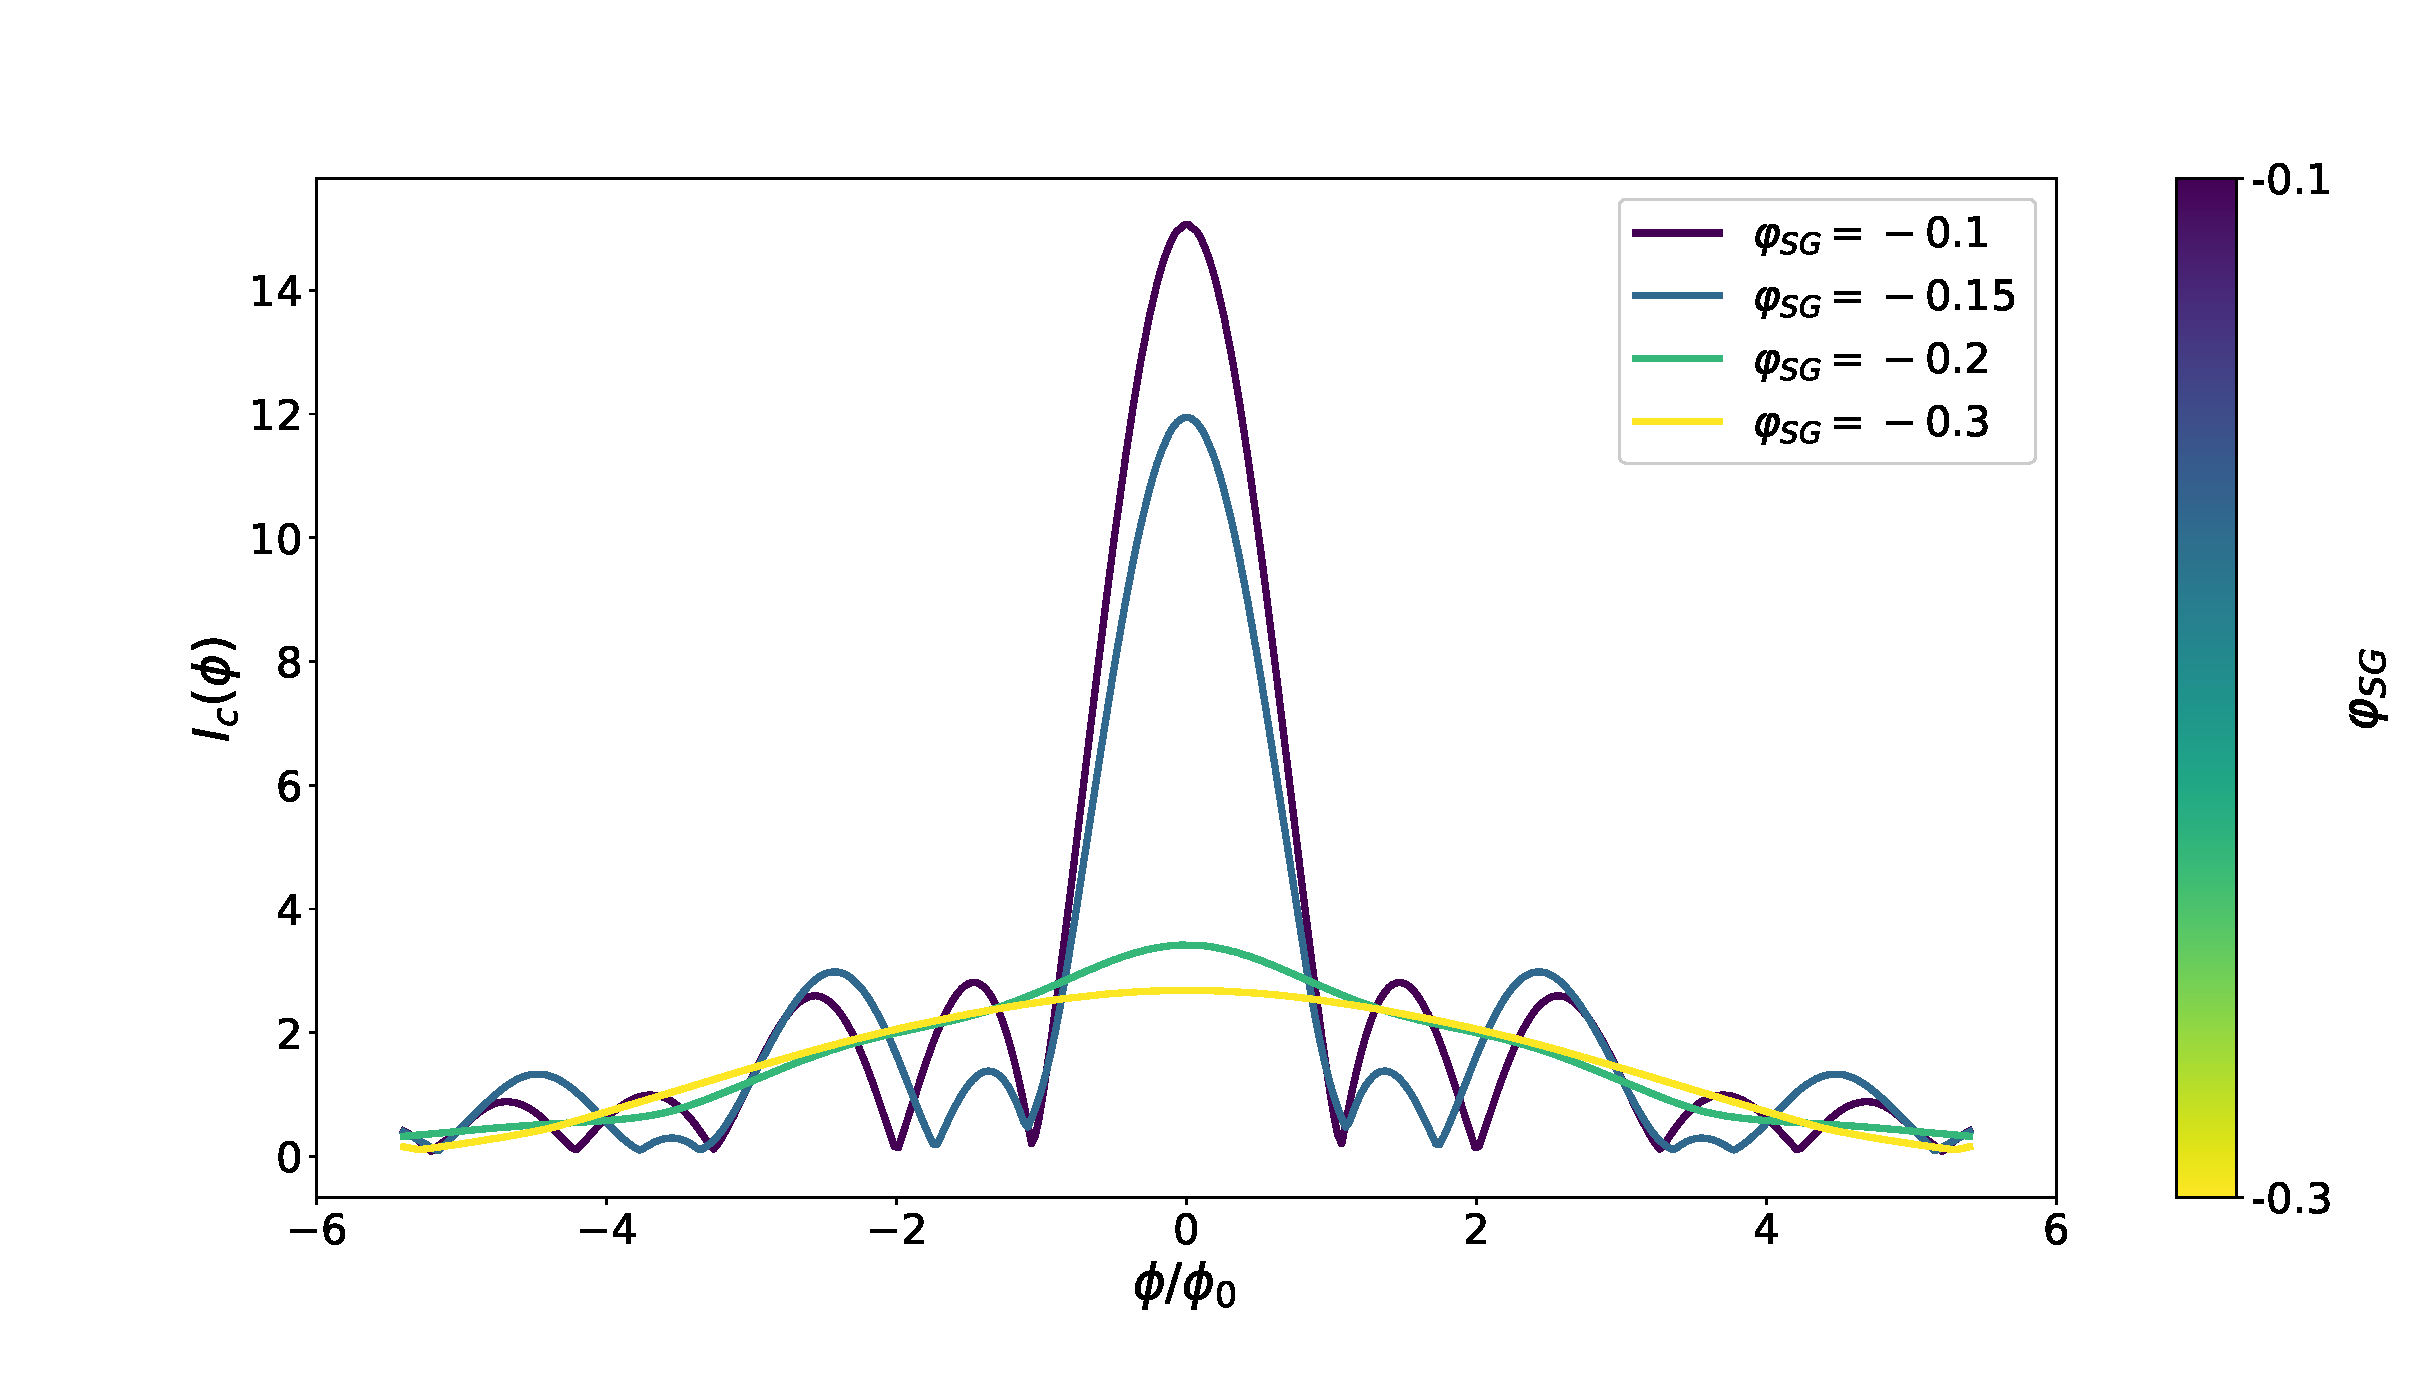
\includegraphics[width=0.8\textwidth]{wg-00-01}
\caption{Supercurrent with increasing splitgate: $\varphi_{SG} \in [0.0, -0.1]$}
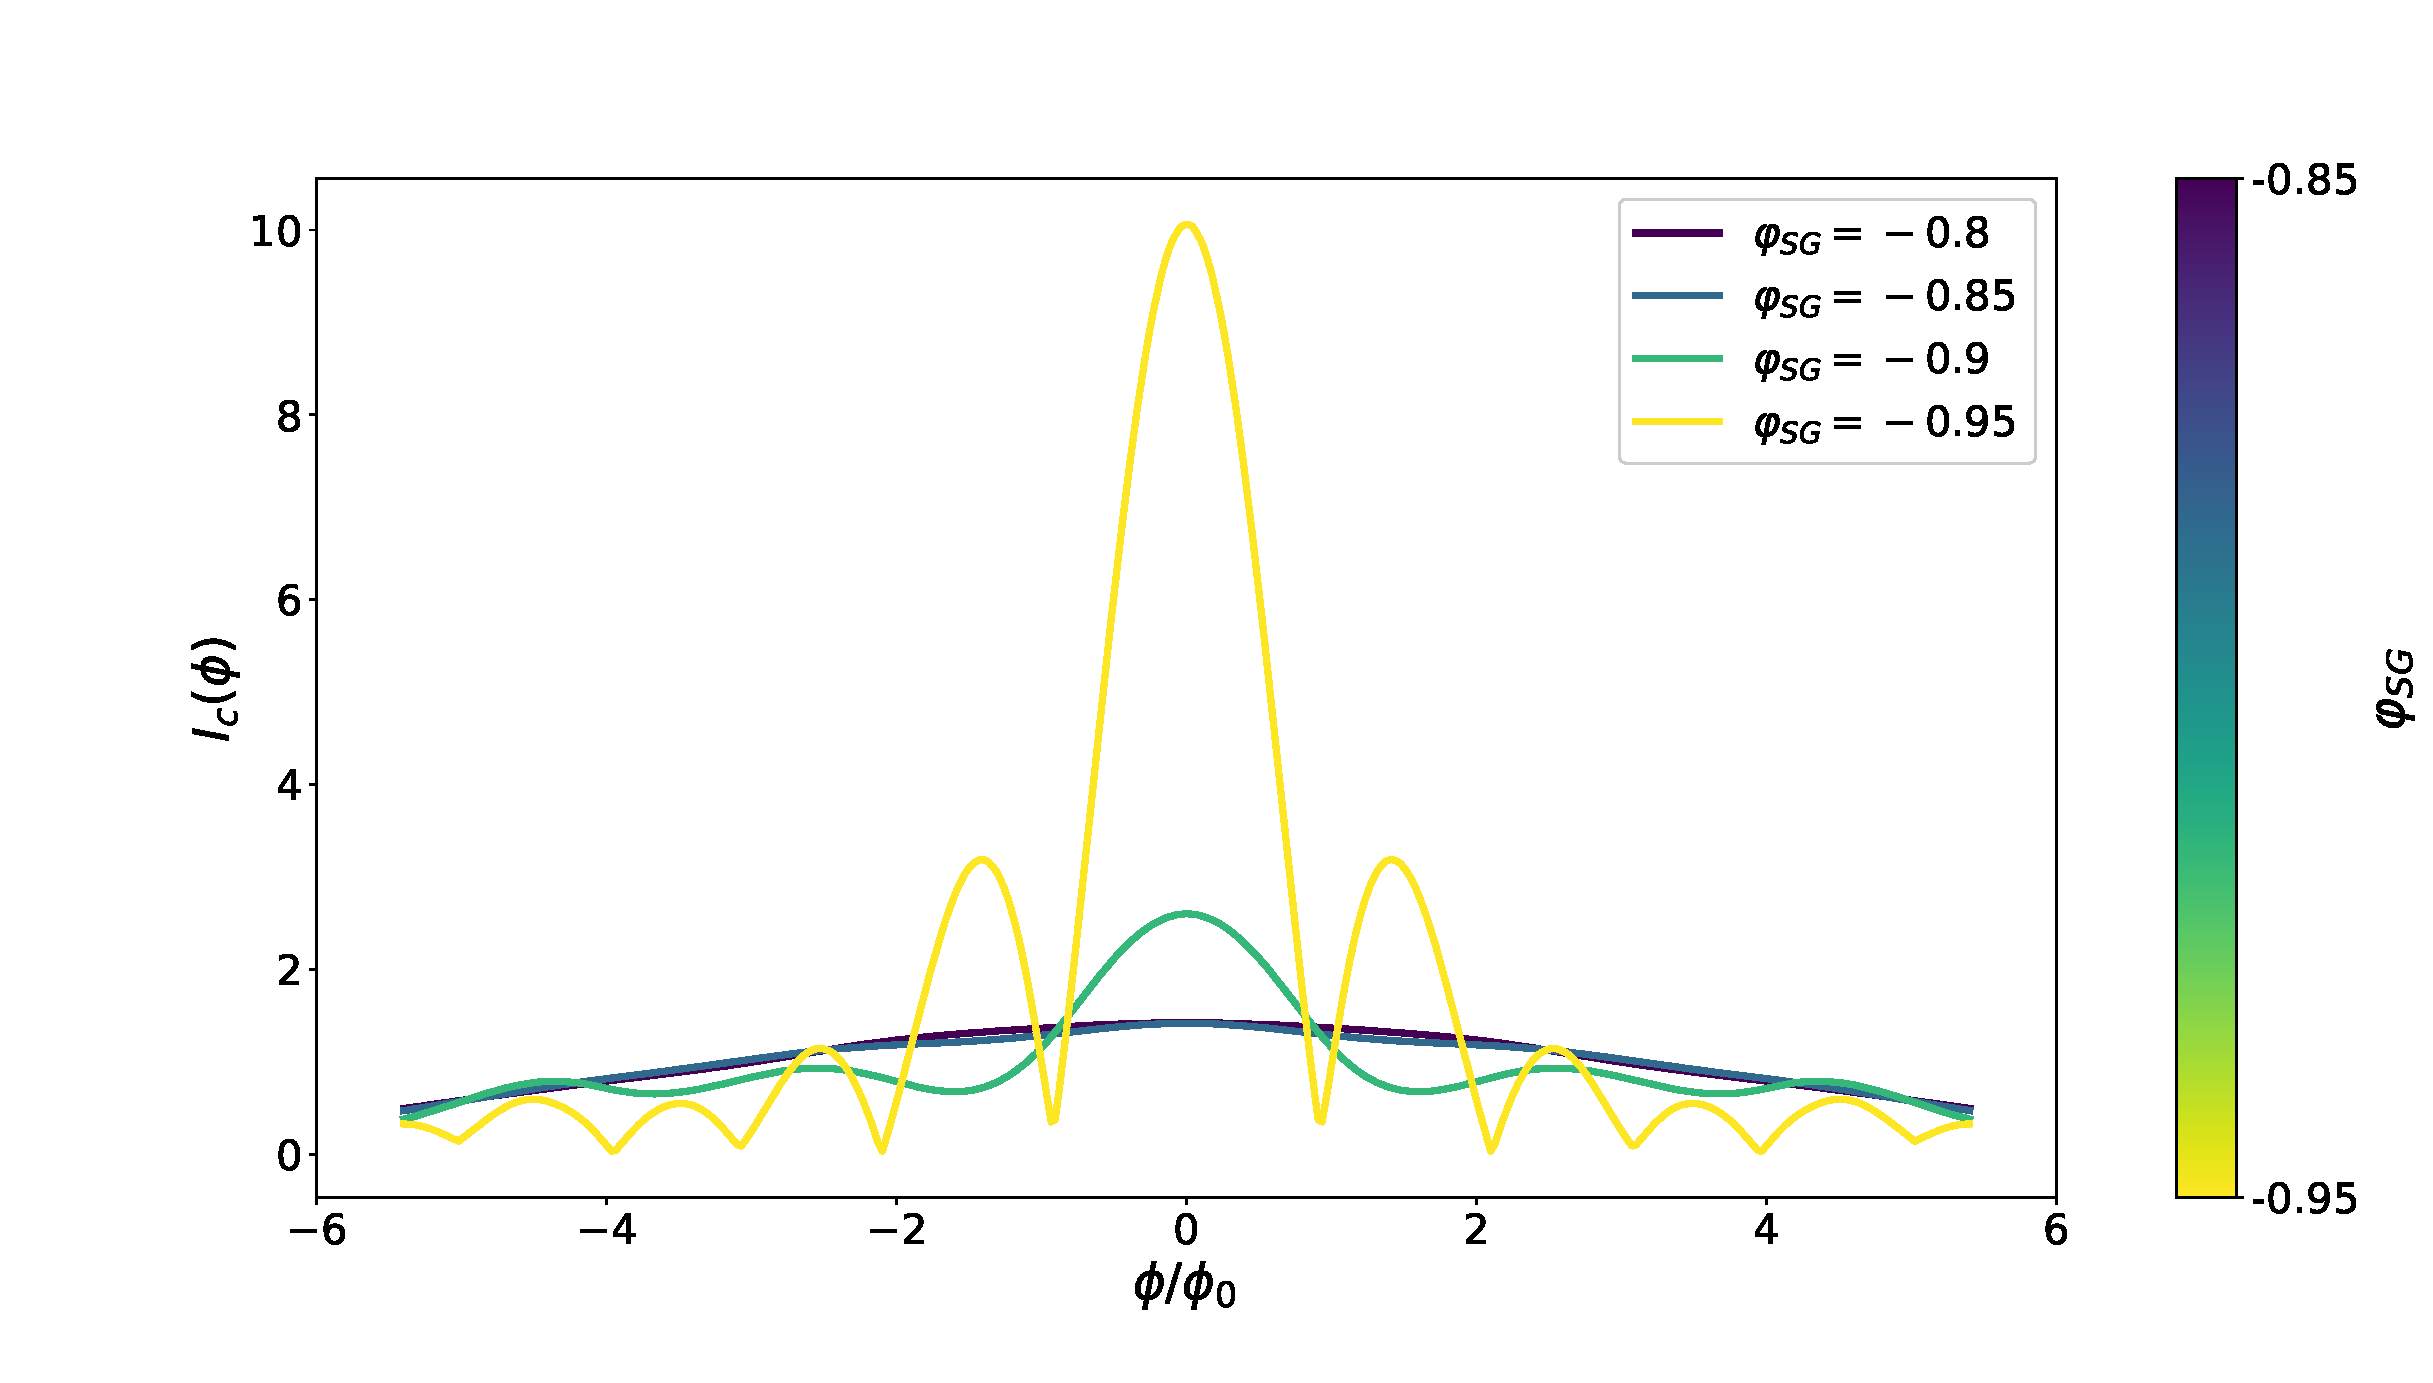
\includegraphics[width=0.8\textwidth]{wg-085-095}
\caption{Supercurrent with increasing splitgate: $\varphi_{SG} \in [-0.5, -0.8]$}
\end{figure}


\end{document}